\documentclass[dvipdfmx,9pt]{beamer}
\usepackage{bxdpx-beamer}
\usepackage{pxjahyper}


% \renewcommand{\kanjifamilydefault}{\gtdefault}
% \setbeamertemplate{navigation symbols}{}
% \usefonttheme{professionalfonts}
% \usetheme{Madrid}


%デザインの選択(省略可)
\usetheme{Luebeck}
%カラーテーマの選択(省略可)
\usecolortheme{orchid}
%フォントテーマの選択(省略可)
\usefonttheme{professionalfonts}
%フレーム内のテーマの選択(省略可)
\useinnertheme{circles}
%フレーム外側のテーマの選択(省略可)
\useoutertheme{infolines}
%しおりの文字化け解消
\usepackage{atbegshi}
\ifnum 42146=\euc"A4A2
\AtBeginShipoutFirst{\special{pdf:tounicode EUC-UCS2}}
\else
\AtBeginShipoutFirst{\special{pdf:tounicode 90ms-RKSJ-UCS2}}
\fi
%ナビゲーションバー非表示
\setbeamertemplate{navigation symbols}{}
%既定をゴシック体に
\renewcommand{\kanjifamilydefault}{\gtdefault}
%タイトル色
\setbeamercolor{title}{fg=structure, bg=}
%フレームタイトル色
\setbeamercolor{frametitle}{fg=structure, bg=}
%スライド番号のみ表示
%\setbeamertemplate{footline}[frame number]
%itemize
\setbeamertemplate{itemize item}{\small\raise0.5pt\hbox{$\bullet$}}
\setbeamertemplate{itemize subitem}{\tiny\raise1.5pt\hbox{$\blacktriangleright$}}
\setbeamertemplate{itemize subsubitem}{\tiny\raise1.5pt\hbox{$\bigstar$}}
% color
\newcommand{\red}[1]{\textcolor{red}{#1}}
\newcommand{\green}[1]{\textcolor{green!40!black}{#1}}
\newcommand{\blue}[1]{\textcolor{blue!80!black}{#1}}

\usepackage{docmute}
\usepackage{graphicx}
\usepackage{dcolumn}
\usepackage{bm}
\usepackage{physics}
\usepackage{amsmath}
\usepackage[version=3]{mhchem}
\usepackage{subfig}
\usepackage{color}
\usepackage{ifthen}
\usepackage{mathtools}
\captionsetup[figure]{font=small,labelfont=bf,justification=raggedright,format=plain}


\newcommand{\exps}[1]{\mathrm{e}^{ #1 }}
\newcommand{\expi}[1]{\exp\pqty{ #1 }}
\newcommand{\exv}[2][t]{\mathbb{E}_{ #1 } \left\lbrack #2 \right\rbrack}


\title{SABR ModelのImplied Volatility}

\author{kakune}
\subject{\LaTeX{}+Beamer}

\begin{document}
\begin{frame}
  \titlepage
\end{frame}

\begin{frame}<beamer>
  \frametitle{Agenda}
  \tableofcontents
\end{frame}

\begin{frame}{Introduction}
  \begin{alertblock}{本スライドの目的と注意}
    \begin{itemize}
      \item 本スライドは、Volatilityが変動するModelにおける、Implied Volatilityの概念・振る舞い・近似式の導出を理解することを目的とする。
      \item 特に近似式の導出は、よい計算練習になる。そのために、天下り的な記述をなるべく避け、発見的に計算が行われる(ように見える)よう工夫した。
      \item もともと手書きノートで行う予定だったが、やたらmessyになってしまったので、補助としてこのスライドを作成した。
      \item すべての確率変数は$T$-Forward measureの下であるとする。
      \item このスライドは、主に N. Zhang "Properties of the SABR model"に基づく。
    \end{itemize}
  \end{alertblock}
\end{frame}

\section{Introduction}
\subsection{Implied Volatility}
\begin{frame}{Introduction}
  \begin{block}{Implied Volatility}
    \begin{itemize}
      \item Black Modelでは、assetのForward価格は、以下のSDEに従う。
            \begin{equation}
              \dd F_{t} = \sigma^{\mathrm{B}} \dd W_{t}
            \end{equation}
      \item このModelを仮定すれば、市場のオプション価格から、quoteするvolを逆算できる。
      \item これを\textbf{Implied Volatility (IV)}と呼ぶ。
    \end{itemize}
  \end{block}
  \begin{block}{Black Modelの限界と改良}
    \begin{itemize}
      \item しかし、実際に計算してみると、オプションのストライクに依存してIVが変化することがわかる。
            \begin{itemize}
              \item Volatility Skew や Volatility Smile。
            \end{itemize}
      \item すなわち、Black Modelは市場を再現できていないことになる。
      \item そこで、よりよいModelとして、Volatilityが変動するModelが考案された。
            \begin{itemize}
              \item \textbf{Local Volatility (LV) Model}: Volが現在価格のdeteministicな関数とするModel。
              \item \textbf{Stochastic Volatility (SV) Model}: Volが確率変動するModel。
            \end{itemize}
    \end{itemize}
  \end{block}
\end{frame}

\subsection{Black Model}
\begin{frame}{Black Model}
  \begin{block}{Model}
    Forward price $F_{t}(T)$が、
    \begin{equation}
      \dd F_{t}(T) = \sigma^{\mathrm{B}} \dd W_{t}
    \end{equation}
    に従うとするModel\footnote{以降、$(T)$はしばしば省略する。}。
    これは解くことができて、 ($s \leq t\leq T$)として$F_{t}(T) = F_{s}(T)\expi{\sigma^{\mathrm{B}}(W_{t} - W_{s})-\frac{\pqty{\sigma^{\mathrm{B}}}^{2}}{2}(t-s)}$となる。
  \end{block}
  \begin{block}{European Call Optionの価格}
    時刻$T>0$に行使し、時刻$\tau >T$で受け取るstrike $K$のeuropean call optionの時刻$t$での価格は、
    \begin{equation}
      C_{t}(T,\tau) = P_{t}(t,\tau)\exv[t]{\pqty{F_{t}(T) - K}^{+}}
    \end{equation}
    ブラウン運動の確率分布を考えて解くと、
    \begin{align}
      C_{t}(T,\tau) & = P_{t}(t,\tau) \pqty{F_{t} N(d_{t}^{+}) - KN(d_{t}^{-})}                                                                  \\
      d_{t}^{\pm}   & = \frac{1}{\sigma^{\mathrm{B}}\sqrt{T-t}}\pqty{\log\pqty{\frac{F_{t}}{K}}\pm\frac{\pqty{\sigma^{\mathrm{B}}}^{2}}{2}(T-t)}
    \end{align}
    この価格は、$\sigma^{\mathrm{B}}$について単調増加である。
  \end{block}
\end{frame}

\section{Local Volatility Model}
\subsection{Modelの概要}
\begin{frame}{Modelの概要}
  \begin{block}{Model}
    Forward price $F_{t}(T)$が、
    \begin{equation}
      \dd F_{t}(T) = \sigma^{\mathrm{loc}}(t,F_{t}(T)) F_{t} \dd W_{t}
    \end{equation}
    に従うとするModel\footnote{C++のコードでは、汎用性のため、係数の$F_{t}$を入れていない。}。ここで、$\sigma^{\mathrm{loc}}$はdeterministicな関数。
  \end{block}
  \begin{block}{European Call Optionの価格}
    当然一般に解くことはできないので、$\sigma^{\mathrm{loc}} = \alpha(t)A(f)/f$、$Q(t,f) = \exv[]{(F_{T} - K)^{+}|F_{t}=f}$として、以下のような手順で解く。
    \begin{enumerate}
      \item Feynman-Kacにより、$Q$の満たす偏微分方程式を求める。
      \item 変数変換を行い、$\tilde{Q}(\tau,x)$とする。
      \item $\tilde{Q},A$に対して漸近展開を行う。
      \item 漸近展開を行った各次数に対して偏微分方程式を導く。
    \end{enumerate}
  \end{block}
\end{frame}

\subsection{IVの漸近形}
\begin{frame}
  \begin{block}{IVの漸近形}
    さらに、Black Modelとの比較を行うことにより、implied volatilityの漸近形を求める。
    \begin{enumerate}
      \setcounter{enumi}{4}
      \item 漸近形を整理して、(実質的に)一変数関数にする。
      \item Black Modelにおける、その変数の値を計算する。
      \item LV Modelでの変数を計算し、それをBlack Modelのものと比較することで、IVを求める。
    \end{enumerate}
    具体的に計算すると、
    \begin{equation}
      \sigma^{\mathrm{IV}} \simeq \sigma^{\mathrm{loc}}\pqty{\frac{f+K}{2}}\pqty{1 + \frac{\sigma^{\mathrm{\mathrm{loc}}~\prime\prime}\pqty{\frac{f+K}{2}}}{\sigma^{\mathrm{loc}}\pqty{\frac{f+K}{2}}}}
    \end{equation}
  \end{block}
\end{frame}

\subsection{Modelの限界}
\begin{frame}{LVの限界}
  \begin{block}{LVの限界}
    Marketで観測されるIVが$\sigma^{\mathrm{M}}(F_{0},K)$であるとする。現在のMarketに合うように最低次を考えて$\sigma^{\mathrm{loc}}$のcalibrationを行うと、
    \begin{equation}
      \sigma^{\mathrm{M}}(F_{0},K) = \sigma^{\mathrm{loc}}\pqty{\frac{F_{0}+K}{2}}
    \end{equation}
    となる。ここで、calibrationの直後にforward priceが$F_{0} \to f$と変化したとしよう。すると、そのときのVolは、
    \begin{equation}
      \sigma^{\mathrm{loc}}\pqty{\frac{f+K}{2}} = \sigma^{\mathrm{M}}(F_{0},K+f-F_{0})
    \end{equation}
    となる。例えば$f>F_{0}$とすれば、Volatility curveは左に動くことになる。これは、期待される動きと逆である(Forward priceが右に動いたのだから、curveも右に動いてほしい)。以上が、LVが将来のVolを再現できないと言われる所以である。
  \end{block}
\end{frame}

\section{SABR Model}
\subsection{Modelの概要}
\begin{frame}{Stochastic Volatility Model}
  \begin{block}{Model}
    Forward price $F_{t}(T)$が、
    \begin{equation}
      \dd F_{t}(T) = \sigma_{t} F_{t} \dd W_{t}
    \end{equation}
    に従うとするModel\footnote{C++のコードでは、汎用性のため、係数の$F_{t}$を入れていない。}。ここで、$\sigma_{t}$はあるSDEに従う確率変数。
  \end{block}
  \begin{block}{SABR Model}
    Forward price $F_{t}(T)$が、
    \begin{align}
      \dd F_{t}(T)                & = \alpha_{t} F_{t}^{\beta} \dd W_{t}^{1} \\
      \dd \alpha_{t}              & = \nu \alpha_{t} \dd W_{t}^{2}           \\
      \dd W_{t}^{1} \dd W_{t}^{2} & = \rho \dd t
    \end{align}
    に従うとするModel。
  \end{block}
\end{frame}

\subsection{IVの漸近形}
\begin{frame}{SABRのIVの漸近形}
  \begin{block}{European Call Option価格導出の概要}
    Volが小さいとして、一般に、
    \begin{align}
      \dd F_{t}      & = \ep \alpha_{t} C(F_{t}) \dd W_{t}^{1} \\
      \dd \alpha_{t} & = \ep \nu \alpha_{t} \dd W_{t}^{2}
    \end{align}
    に対して、Option価格を以下のように導く。
    \begin{enumerate}
      \item $F_{t},\alpha_{t}$の同時確率分布$p$について、Focker-Planckの議論でPDEを導く。
      \item Option価格を、$p$のあるの汎関数$P$で表す。
      \item この$P$を変数変換と漸近展開を繰り返して解く。
      \item $P$を用いてOption価格の一般式を出す。
    \end{enumerate}
  \end{block}
\end{frame}
\begin{frame}{SABRのIVの漸近形}
  \begin{block}{IVの導出の概要}
    \begin{enumerate}
      \setcounter{enumi}{4}
      \item Normal Model $C(f) = 1, \ep\alpha_{t} = \sigma^{\mathrm{N}},\nu = 0$に対して漸近展開形を求める。
      \item Black Model $C(f) = f, \alpha_{t} = \sigma^{\mathrm{B}},\nu = 0$に対して漸近展開形を求め、前項の内容と比較して対応する$\sigma^{\mathrm{N,B}}$を求める。
      \item SABR Modelに対しても同様にして、$\sigma^{\mathrm{N,SABR}}$を求める。
      \item $\sigma^{\mathrm{N,SABR}} = \sigma^{\mathrm{N,B}}$を解いて、IVを求める。
    \end{enumerate}
  \end{block}
\end{frame}

\begin{frame}{SABRのIVの漸近形}
  \begin{block}{変数変換の流れ}
    $\raise0.2ex\hbox{\textcircled{\scriptsize{3}}}$について、繰り返し変数変換が行われるので、まとめておく。
    \begin{enumerate}
      \setbeamertemplate{enumerate item}{(\arabic{enumi})}
      \item
            \begin{equation}
              P(\tau ; f,\alpha,K) := \int_{\infty}^{\infty} A^{2} p(t,f,\alpha ; t + \tau ,K,A) \dd A
            \end{equation}
            は次のPDEを満たす︰
            \begin{equation}
              \pdv{P}{\tau} = \frac{\ep^{2}\alpha^{2}C(f)^{2}}{2}\pdv[2]{P}{f} + \ep^{2} \rho \nu \alpha^{2} C(f) \pdv{P}{f}{\alpha} + \frac{\ep^{2}\nu^{2}\alpha^{2}}{2}\pdv[2]{P}{\alpha}
            \end{equation}
      \item
            \begin{equation}
              z = \frac{1}{\ep\alpha}\int^{f}_{K}\frac{\dd g}{C(g)} , \quad \hat{P}(\tau,z,\alpha) := \frac{\ep C(K)}{\alpha} P(\tau,f,\alpha,K)
            \end{equation}
      \item \begin{equation}
              H(\tau,z,\alpha) := \sqrt{\frac{C(K)}{C(f)}}\hat{P}(\tau,z,\alpha)
            \end{equation}
    \end{enumerate}
  \end{block}
\end{frame}

\begin{frame}{SABRのIVの漸近形}
  \begin{block}{変数変換の流れ(続き)}
    \begin{enumerate}
      \setbeamertemplate{enumerate item}{(\arabic{enumi})}
      \setcounter{enumi}{3}
      \item
            \begin{equation}
              \hat{H}(\tau,z,\alpha) := \expi{-\frac{\ep^{2}\rho\nu\alpha b^{(1)}z^{2}}{4}}H(\tau,z,\alpha)
            \end{equation}
      \item
            \begin{equation}
              x := \frac{1}{\ep\nu}\int_{0}^{\ep\nu z}\frac{\dd \zeta}{I(\zeta)}, \quad
              I(\zeta) := \sqrt{1 - 2\rho\zeta + \zeta^{2}}, \quad
              Q(\tau, x) := \frac{\hat{H}(\tau,z,\alpha)}{\sqrt{I(\ep\nu z(x))}}
            \end{equation}
    \end{enumerate}
  \end{block}
\end{frame}


\begin{frame}{SABRのIVの漸近形}
  \begin{block}{SABRのIV}
    最終的に、求めるべきImplied (Normal) Volatilityは、
    \begin{equation}
      \sigma^{\mathrm{IV}} \simeq
      \frac{\alpha}{(fK)^{(1-\beta)/2}}
      \frac{1 + \left( \frac{(1-\beta)^{2}\alpha^{2}}{24(fK)^{1-\beta}}
        + \frac{\rho\beta\nu\alpha}{4(fK)^{(1-\beta)/2}}
        + \frac{(2-3\rho^{2})\nu^{2}}{24}\right)\tau^{\mathrm{ex}}}{1 + \frac{(1-\beta)^{2}}{24}
        \left(\log \frac{f}{K}\right)^{2}
        + \frac{(1-\beta)^{4}}{1920}\left(\log \frac{f}{K}\right)^{4}}
      \frac{\zeta}{\chi(\zeta)}
    \end{equation}
    \begin{equation}
      \begin{split}
        \sigma^{\mathrm{INV}} & \simeq
        \alpha(fK)^{\beta/2}
        \frac{1 + \frac{1}{24}
          \left(\log \frac{f}{K}\right)^{2}
          + \frac{1}{1920}\left(\log \frac{f}{K}\right)^{4}}{1 + \frac{(1-\beta)^{2}}{24}
          \left(\log \frac{f}{K}\right)^{2}
          + \frac{(1-\beta)^{4}}{1920}\left(\log \frac{f}{K}\right)^{4}}
        \frac{\zeta}{\chi(\zeta)} \\
        & ~\times \pqty{
          1 + \left( \frac{-\beta(2-\beta)\alpha^{2}}{24(fK)^{1-\beta}}
          + \frac{\rho\beta\nu\alpha}{4(fK)^{(1-\beta)/2}}
          + \frac{(2-3\rho^{2})\nu^{2}}{24}\right)\tau^{\mathrm{ex}}
        }
      \end{split}
    \end{equation}
    \begin{equation}
      \zeta = \frac{\nu}{\alpha}(fK)^{(1-\beta)/2}\log \frac{f}{K}, \qquad \chi(\zeta) = \log \pqty{ \frac{\sqrt{1 - 2\rho\zeta + \zeta^{2}} - \rho + \zeta}{1-\rho}}
    \end{equation}
  \end{block}
\end{frame}

\subsection{IVのパラメータ依存性}
\begin{frame}{SABR IVのパラメータ依存性}
  めでたく漸近形が出たところで、パラメータ$\alpha(=\alpha_{0}),\beta,\rho,\nu$がそれぞれどういう意味を持つか理解しておこう。\\
  まず、$\alpha$はVolの初期値であり、IVの全体の水準を定める。\\
  $\beta$はスマイルの(backgroundの)傾きに影響する。図の通り(ただし、水準感が合うように$\alpha$を調整している)。

  \begin{figure}
    \begin{minipage}[b]{0.48\linewidth}
      \raggedleft
      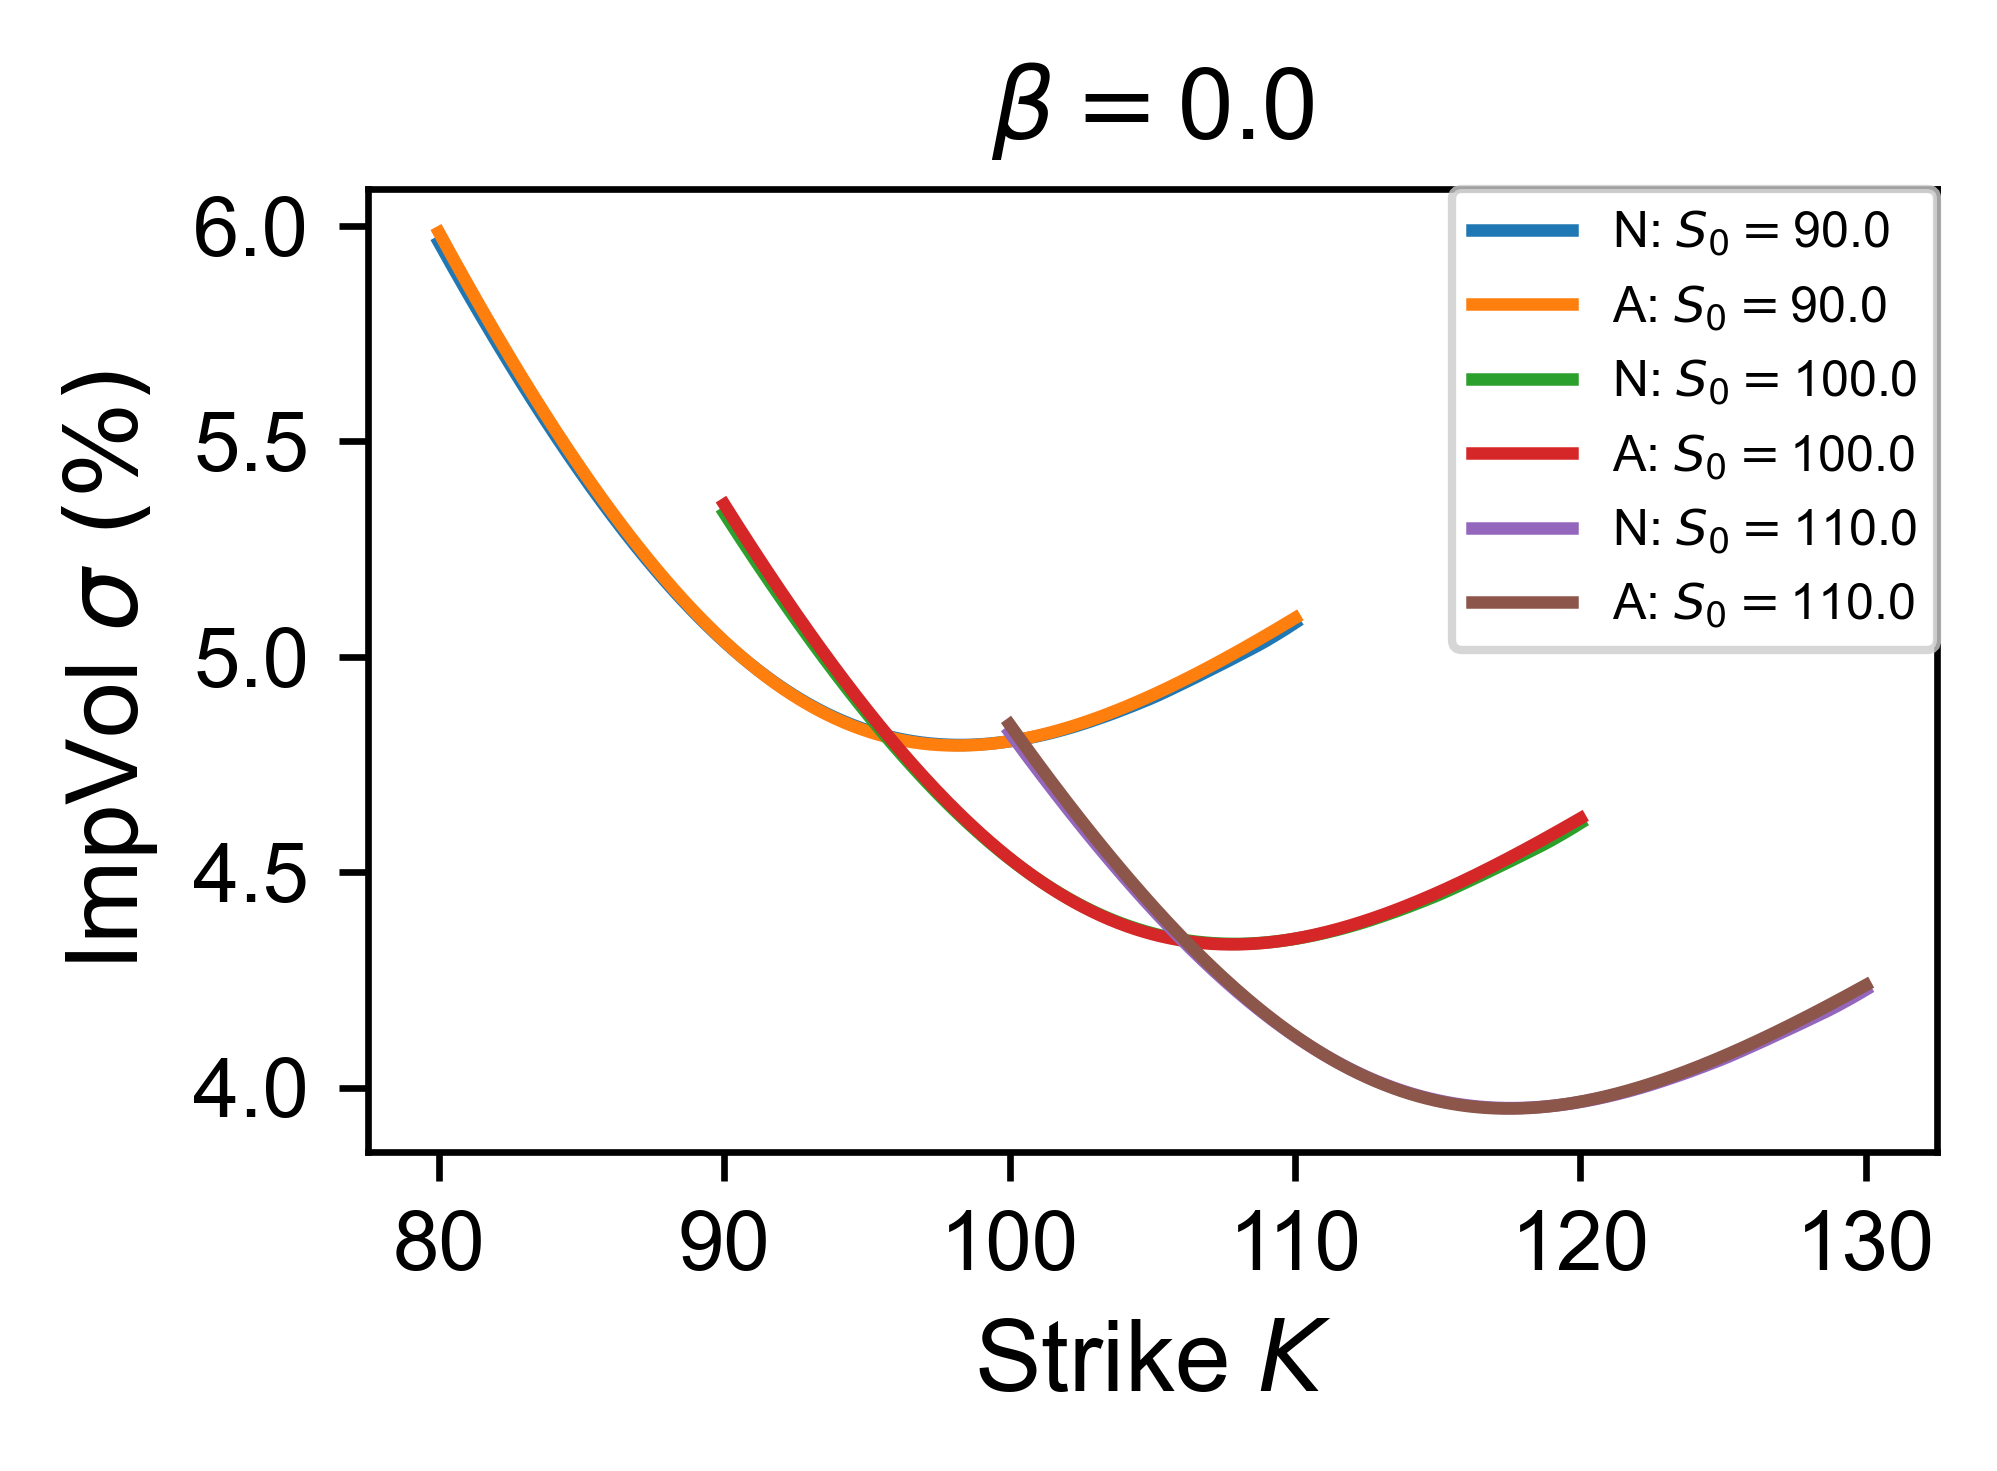
\includegraphics[width=0.7\linewidth]{image/beta/SABR_graph_0.0.png}
    \end{minipage}
    \hfill
    \begin{minipage}[b]{0.48\linewidth}
      \raggedright
      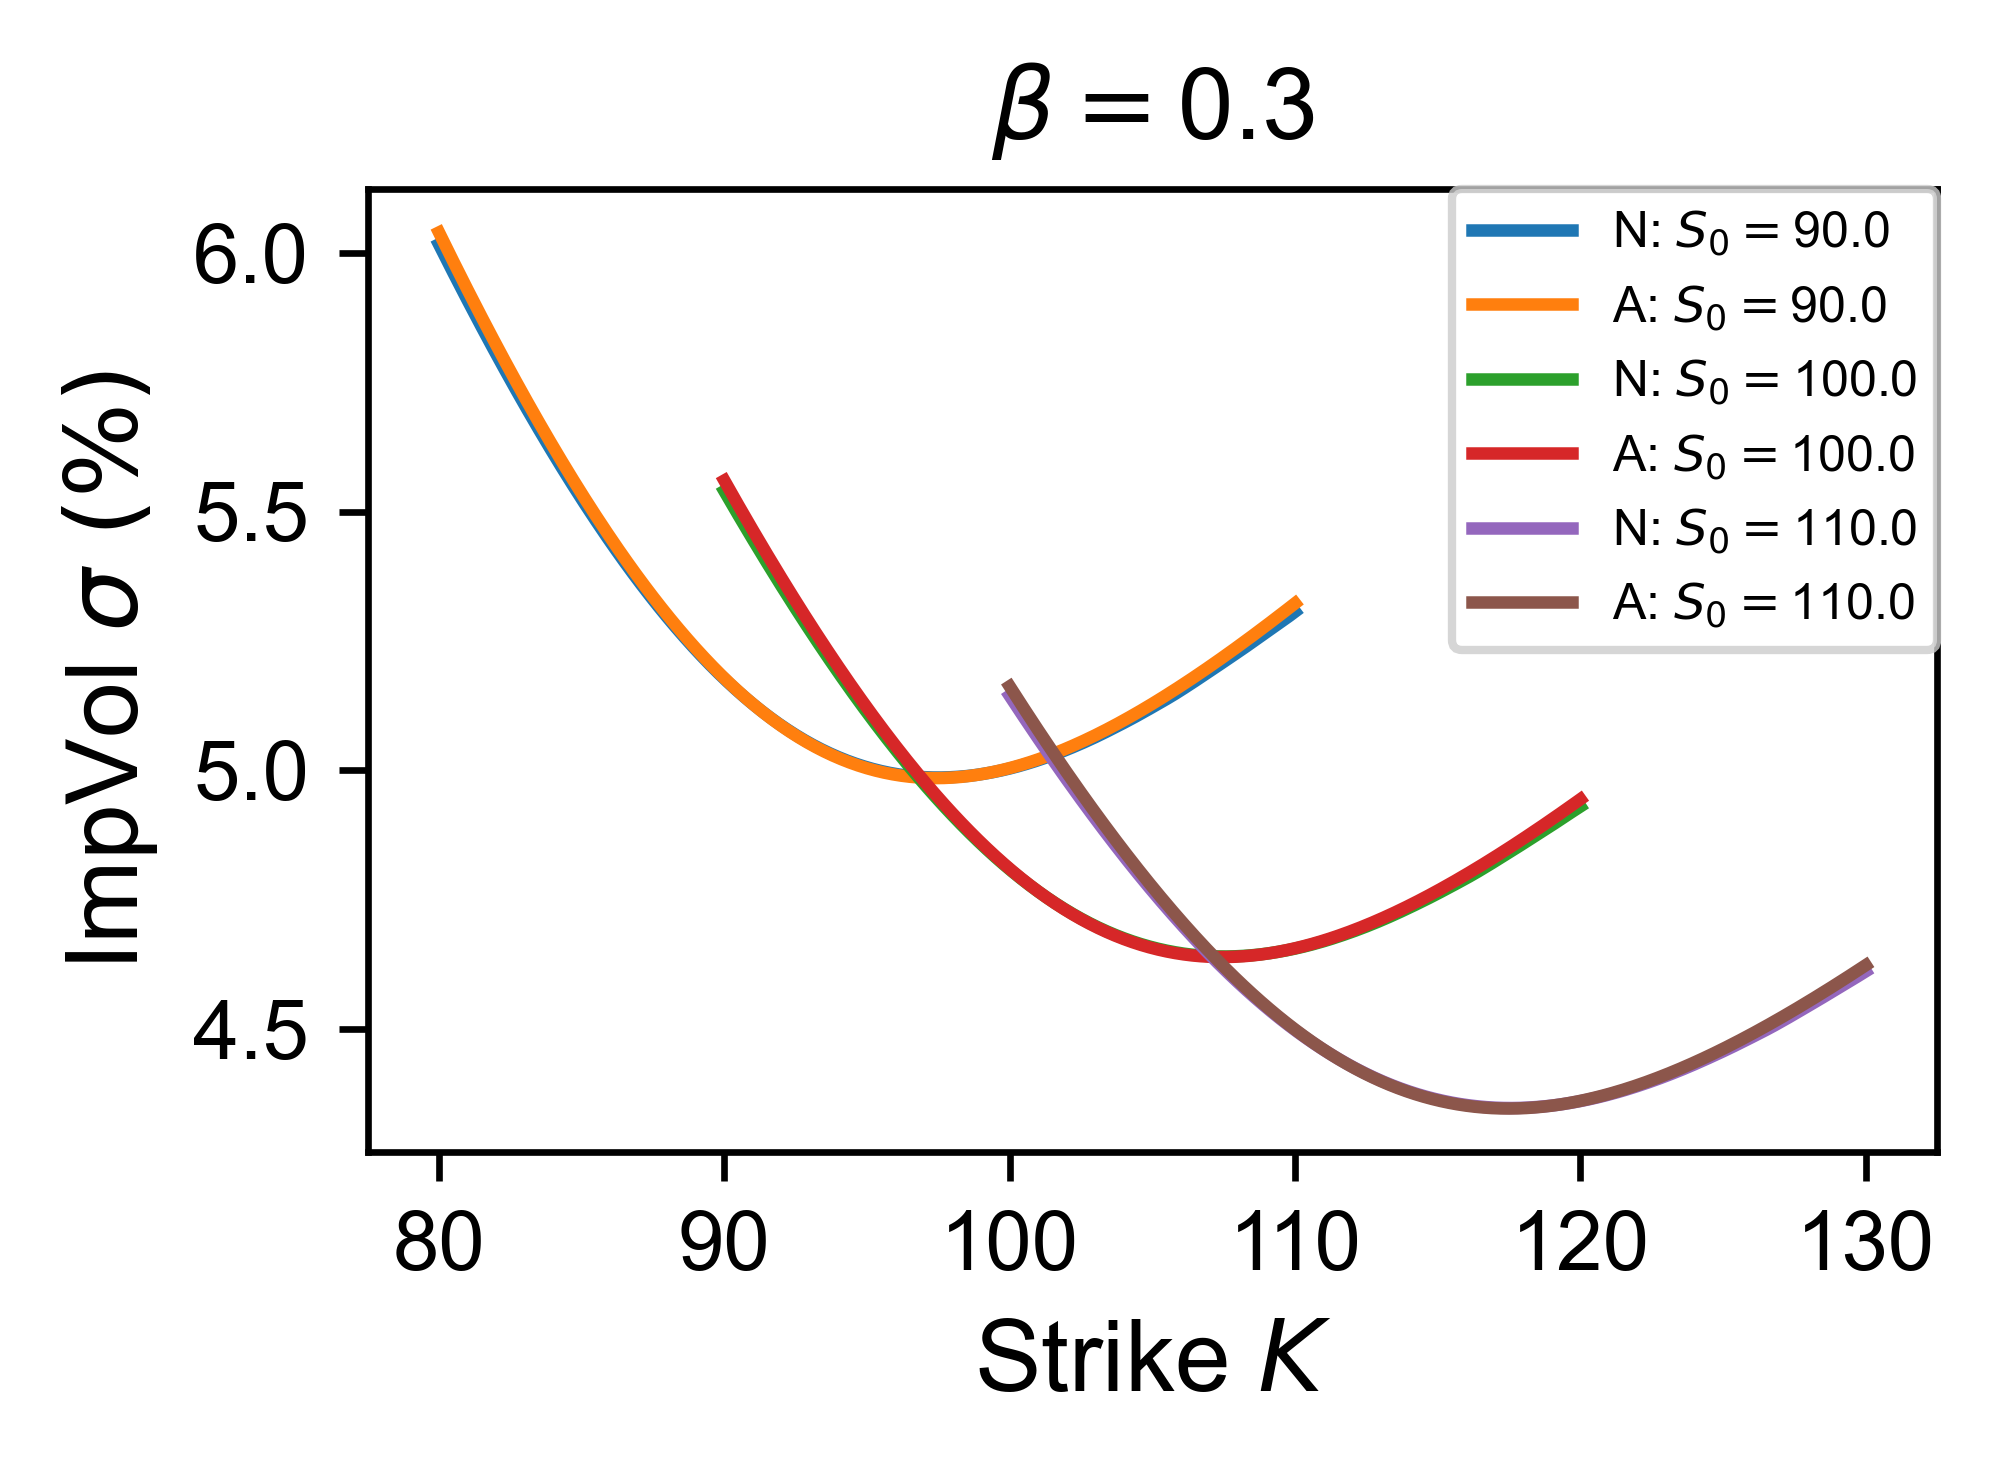
\includegraphics[width=0.7\linewidth]{image/beta/SABR_graph_0.3.png}
    \end{minipage}
  \end{figure}

  \begin{figure}
    \begin{minipage}[b]{0.48\linewidth}
      \raggedleft
      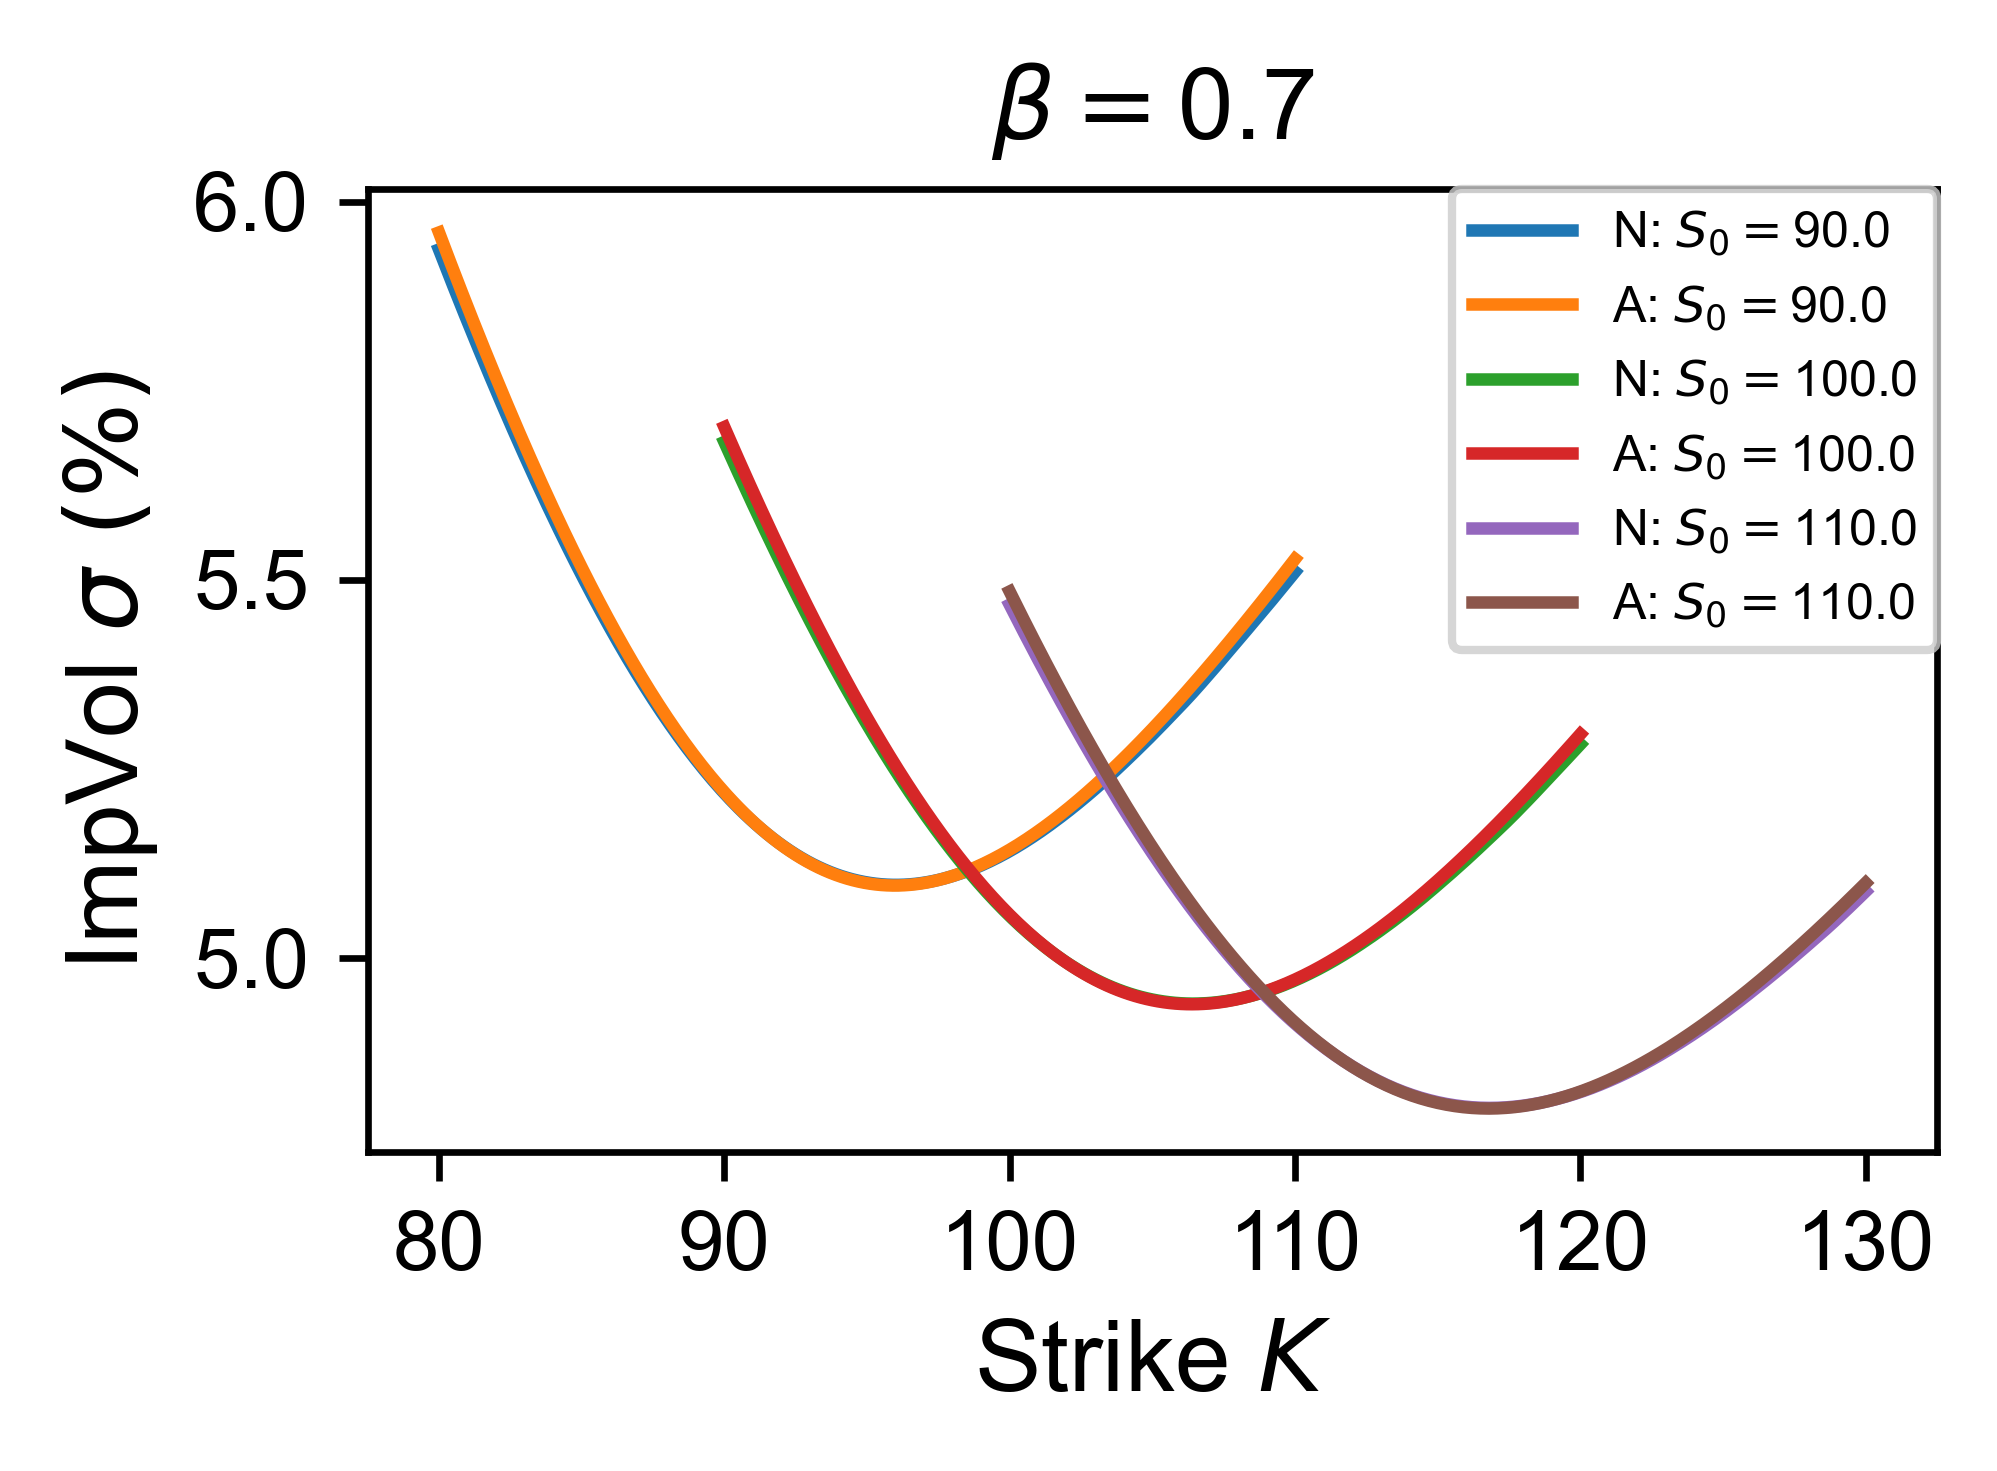
\includegraphics[width=0.7\linewidth]{image/beta/SABR_graph_0.7.png}
    \end{minipage}
    \hfill
    \begin{minipage}[b]{0.48\linewidth}
      \raggedright
      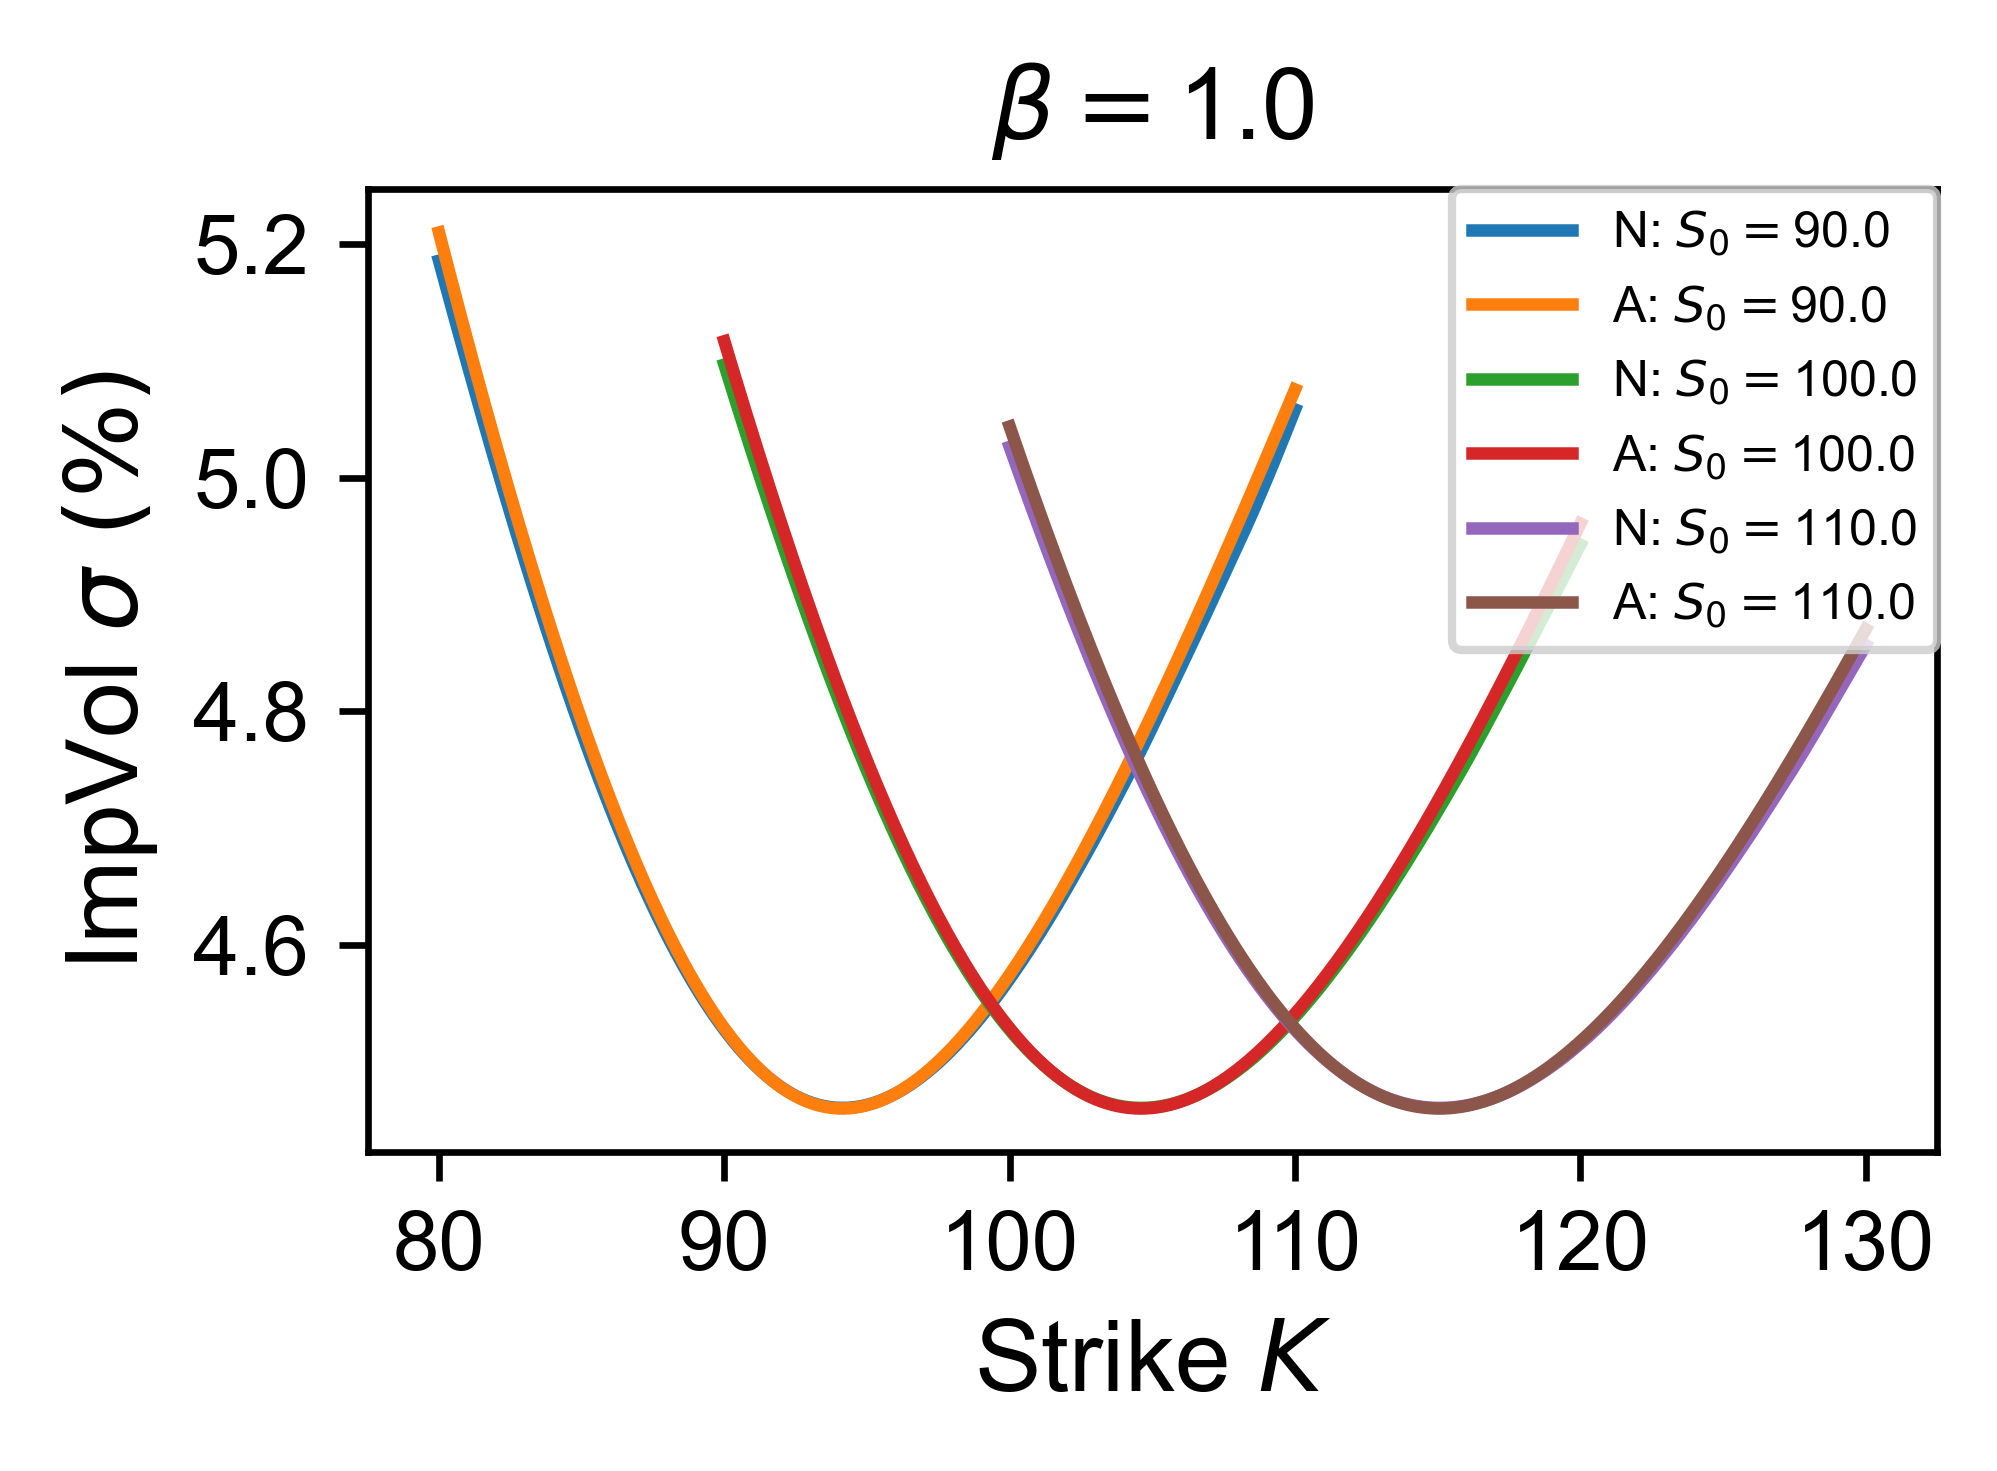
\includegraphics[width=0.7\linewidth]{image/beta/SABR_graph_1.0.png}
    \end{minipage}
  \end{figure}

\end{frame}

\begin{frame}{SABR IVのパラメータ依存性}
  $\nu$はVolの変動幅を表し、スマイルの曲率に影響する。
  \begin{figure}
    \begin{minipage}[b]{0.48\linewidth}
      \raggedleft
      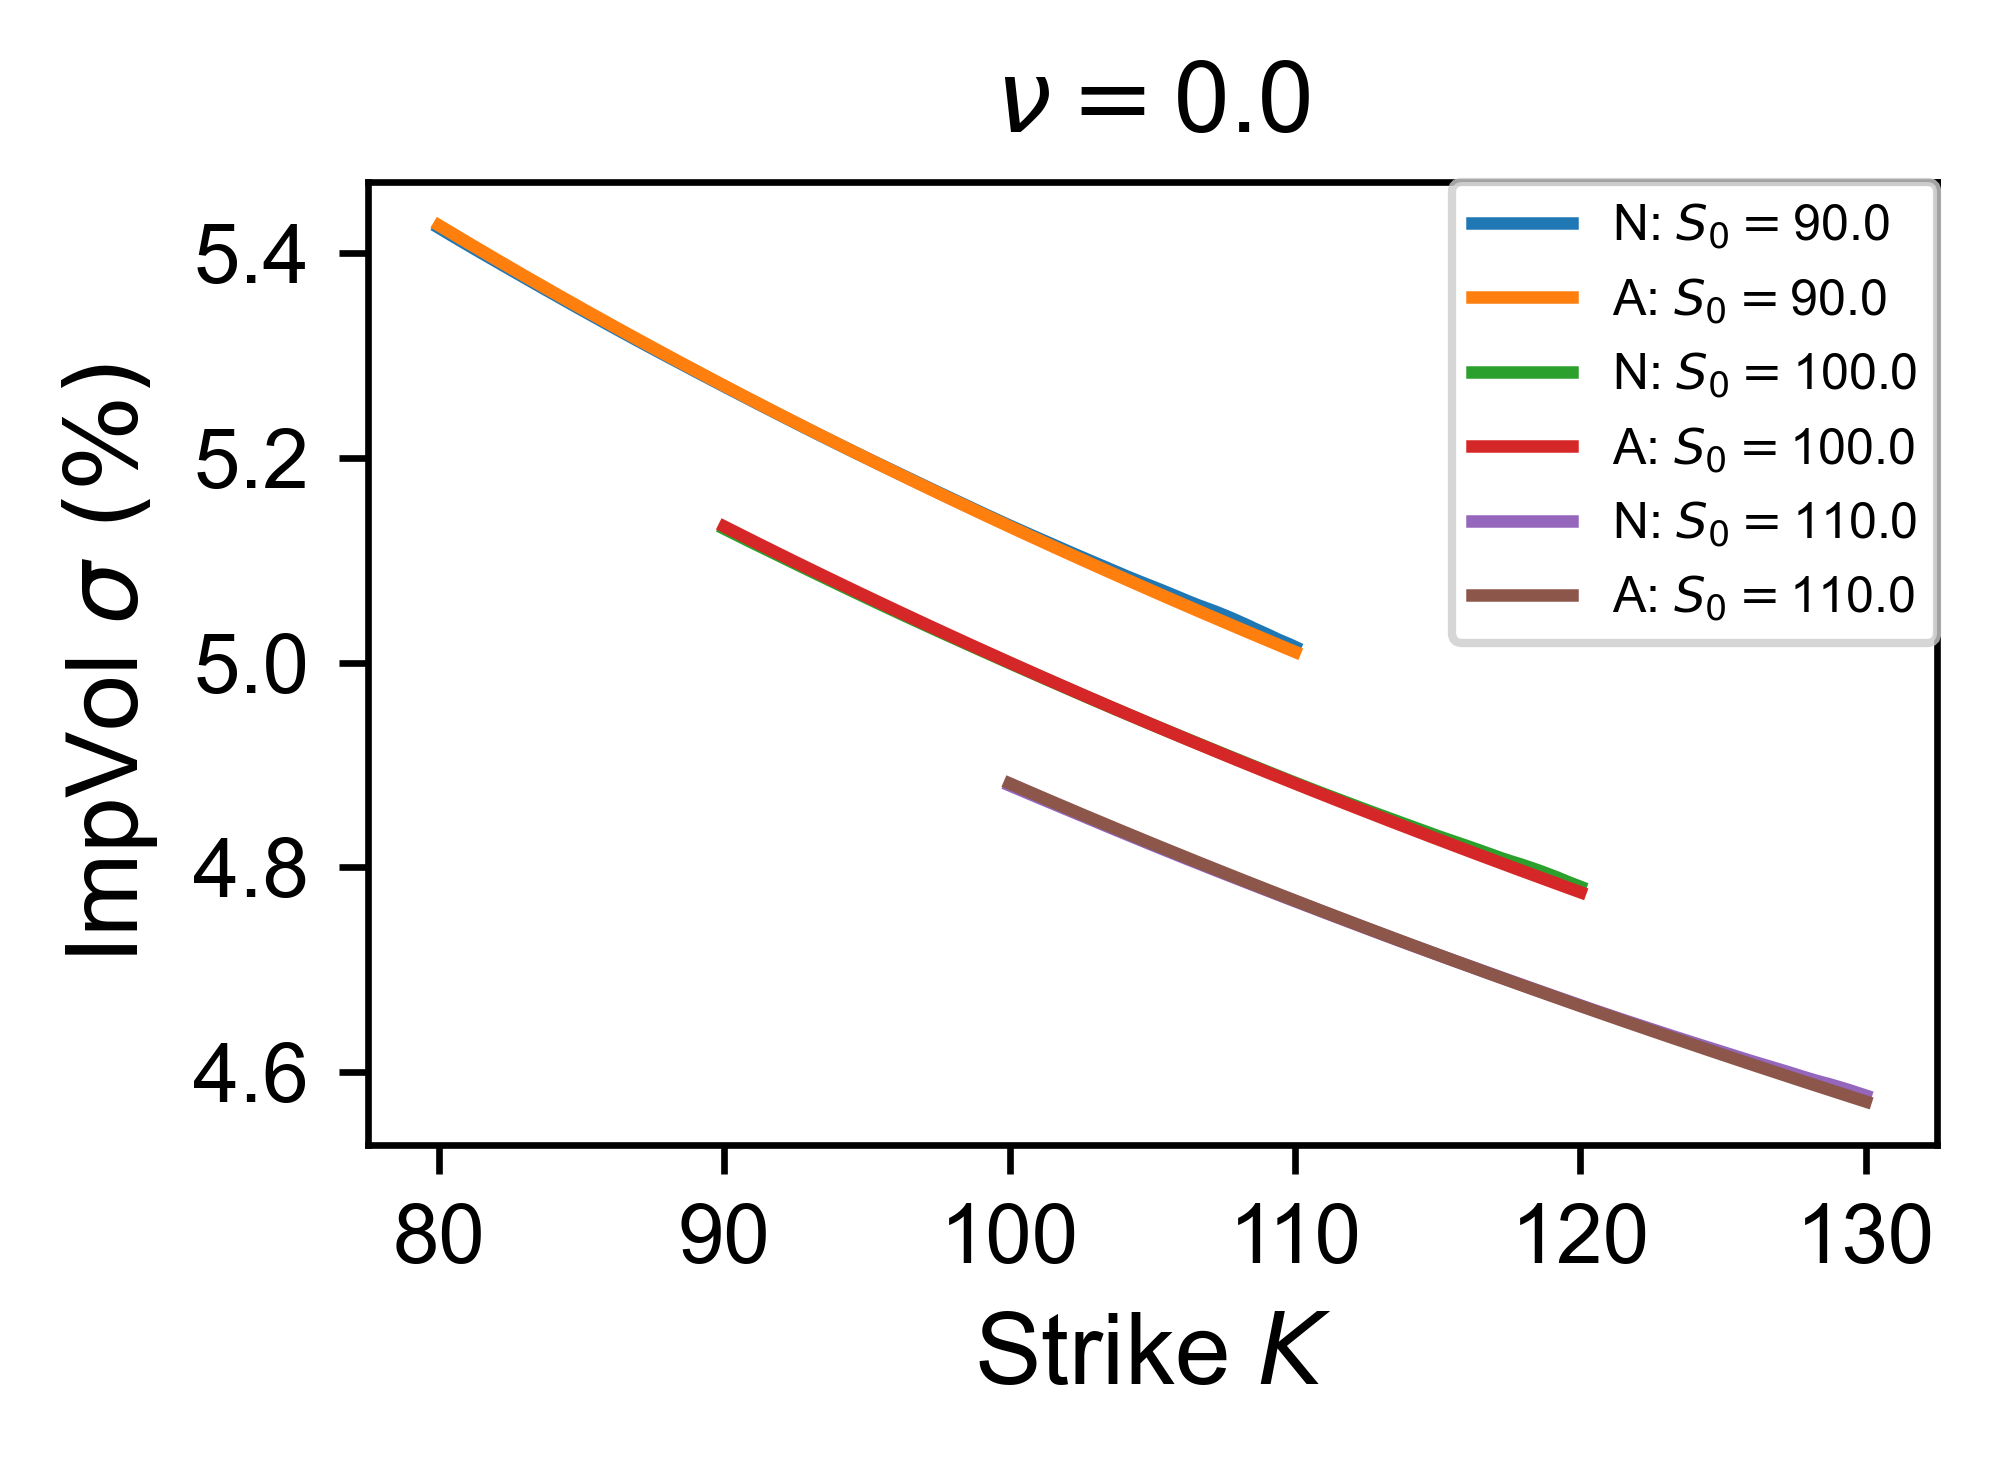
\includegraphics[width=0.7\linewidth]{image/volvol/SABR_graph_0.0.png}
    \end{minipage}
    \hfill
    \begin{minipage}[b]{0.48\linewidth}
      \raggedright
      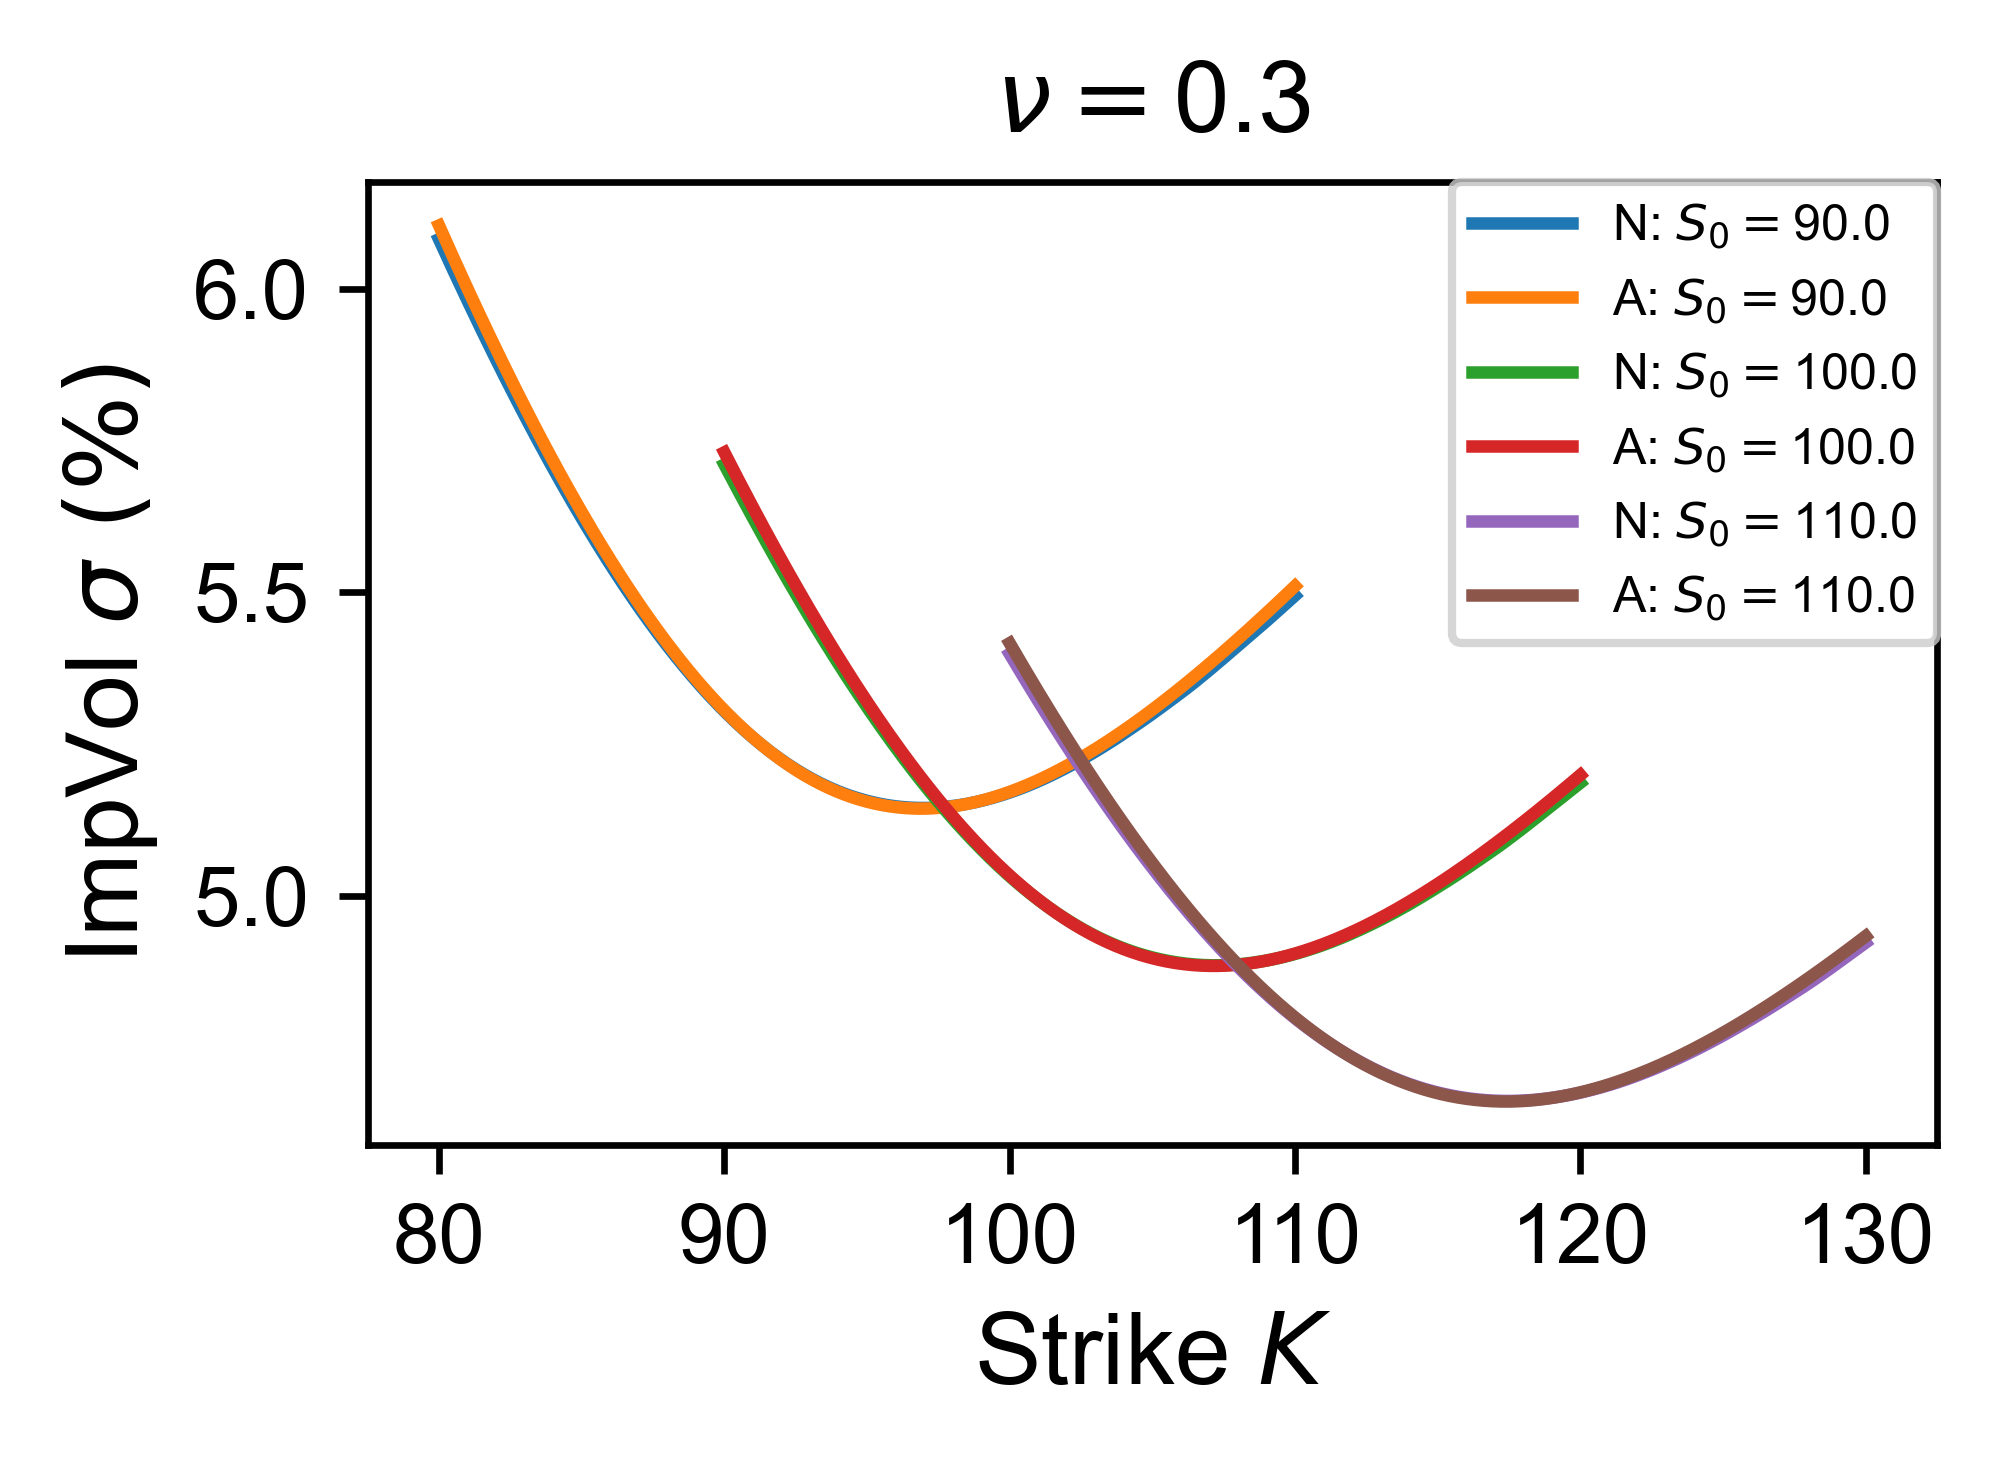
\includegraphics[width=0.7\linewidth]{image/volvol/SABR_graph_0.3.png}
    \end{minipage}
  \end{figure}

  \begin{figure}
    \begin{minipage}[b]{0.48\linewidth}
      \raggedleft
      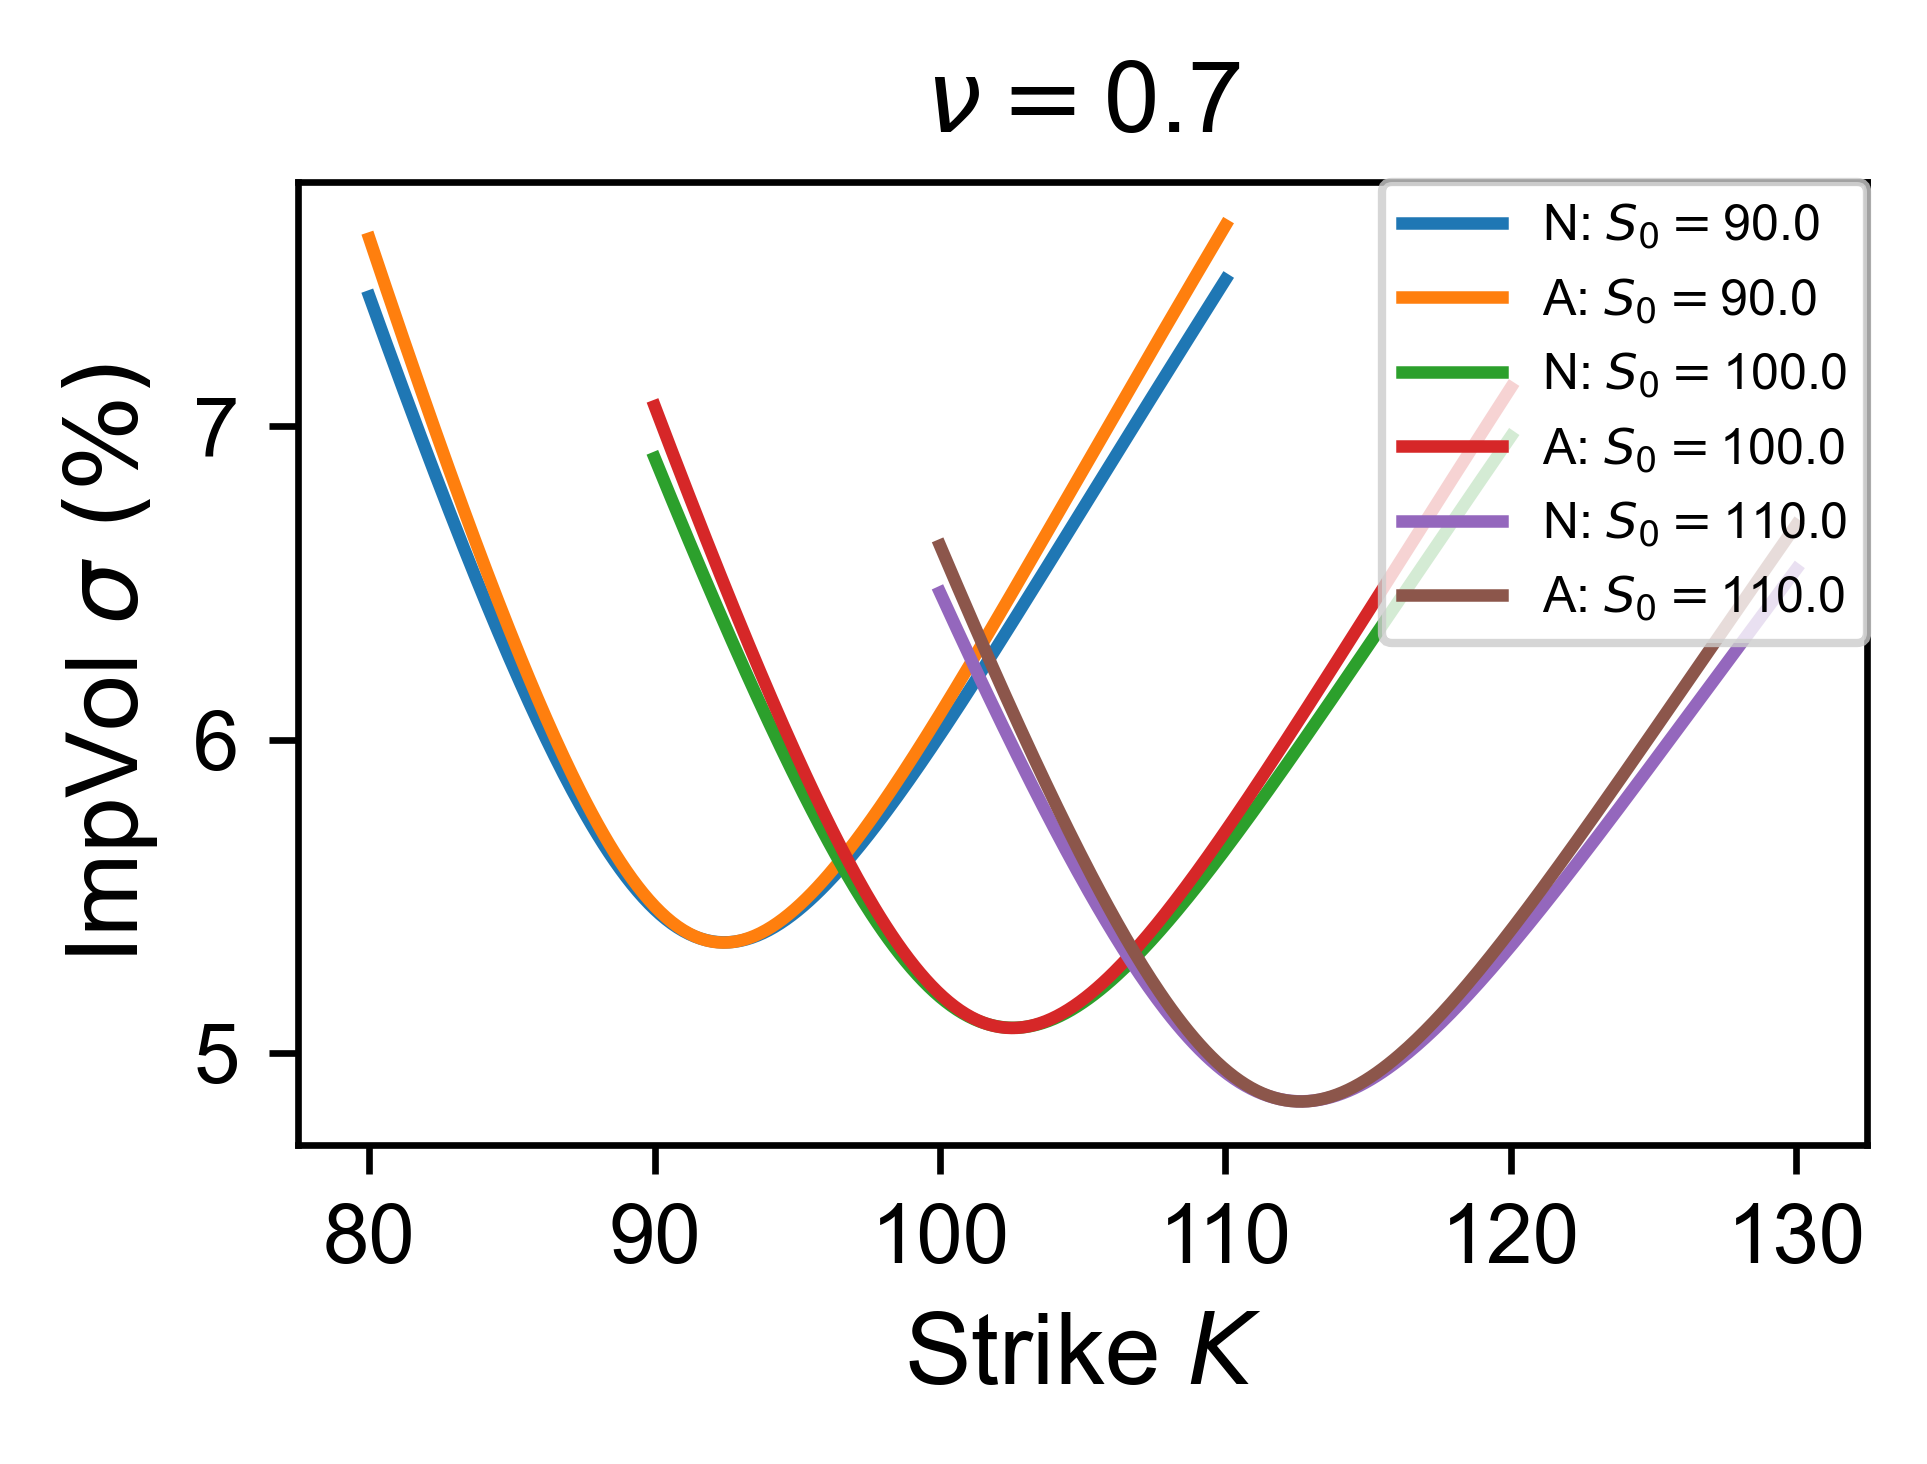
\includegraphics[width=0.7\linewidth]{image/volvol/SABR_graph_0.7.png}
    \end{minipage}
    \hfill
    \begin{minipage}[b]{0.48\linewidth}
      \raggedright
      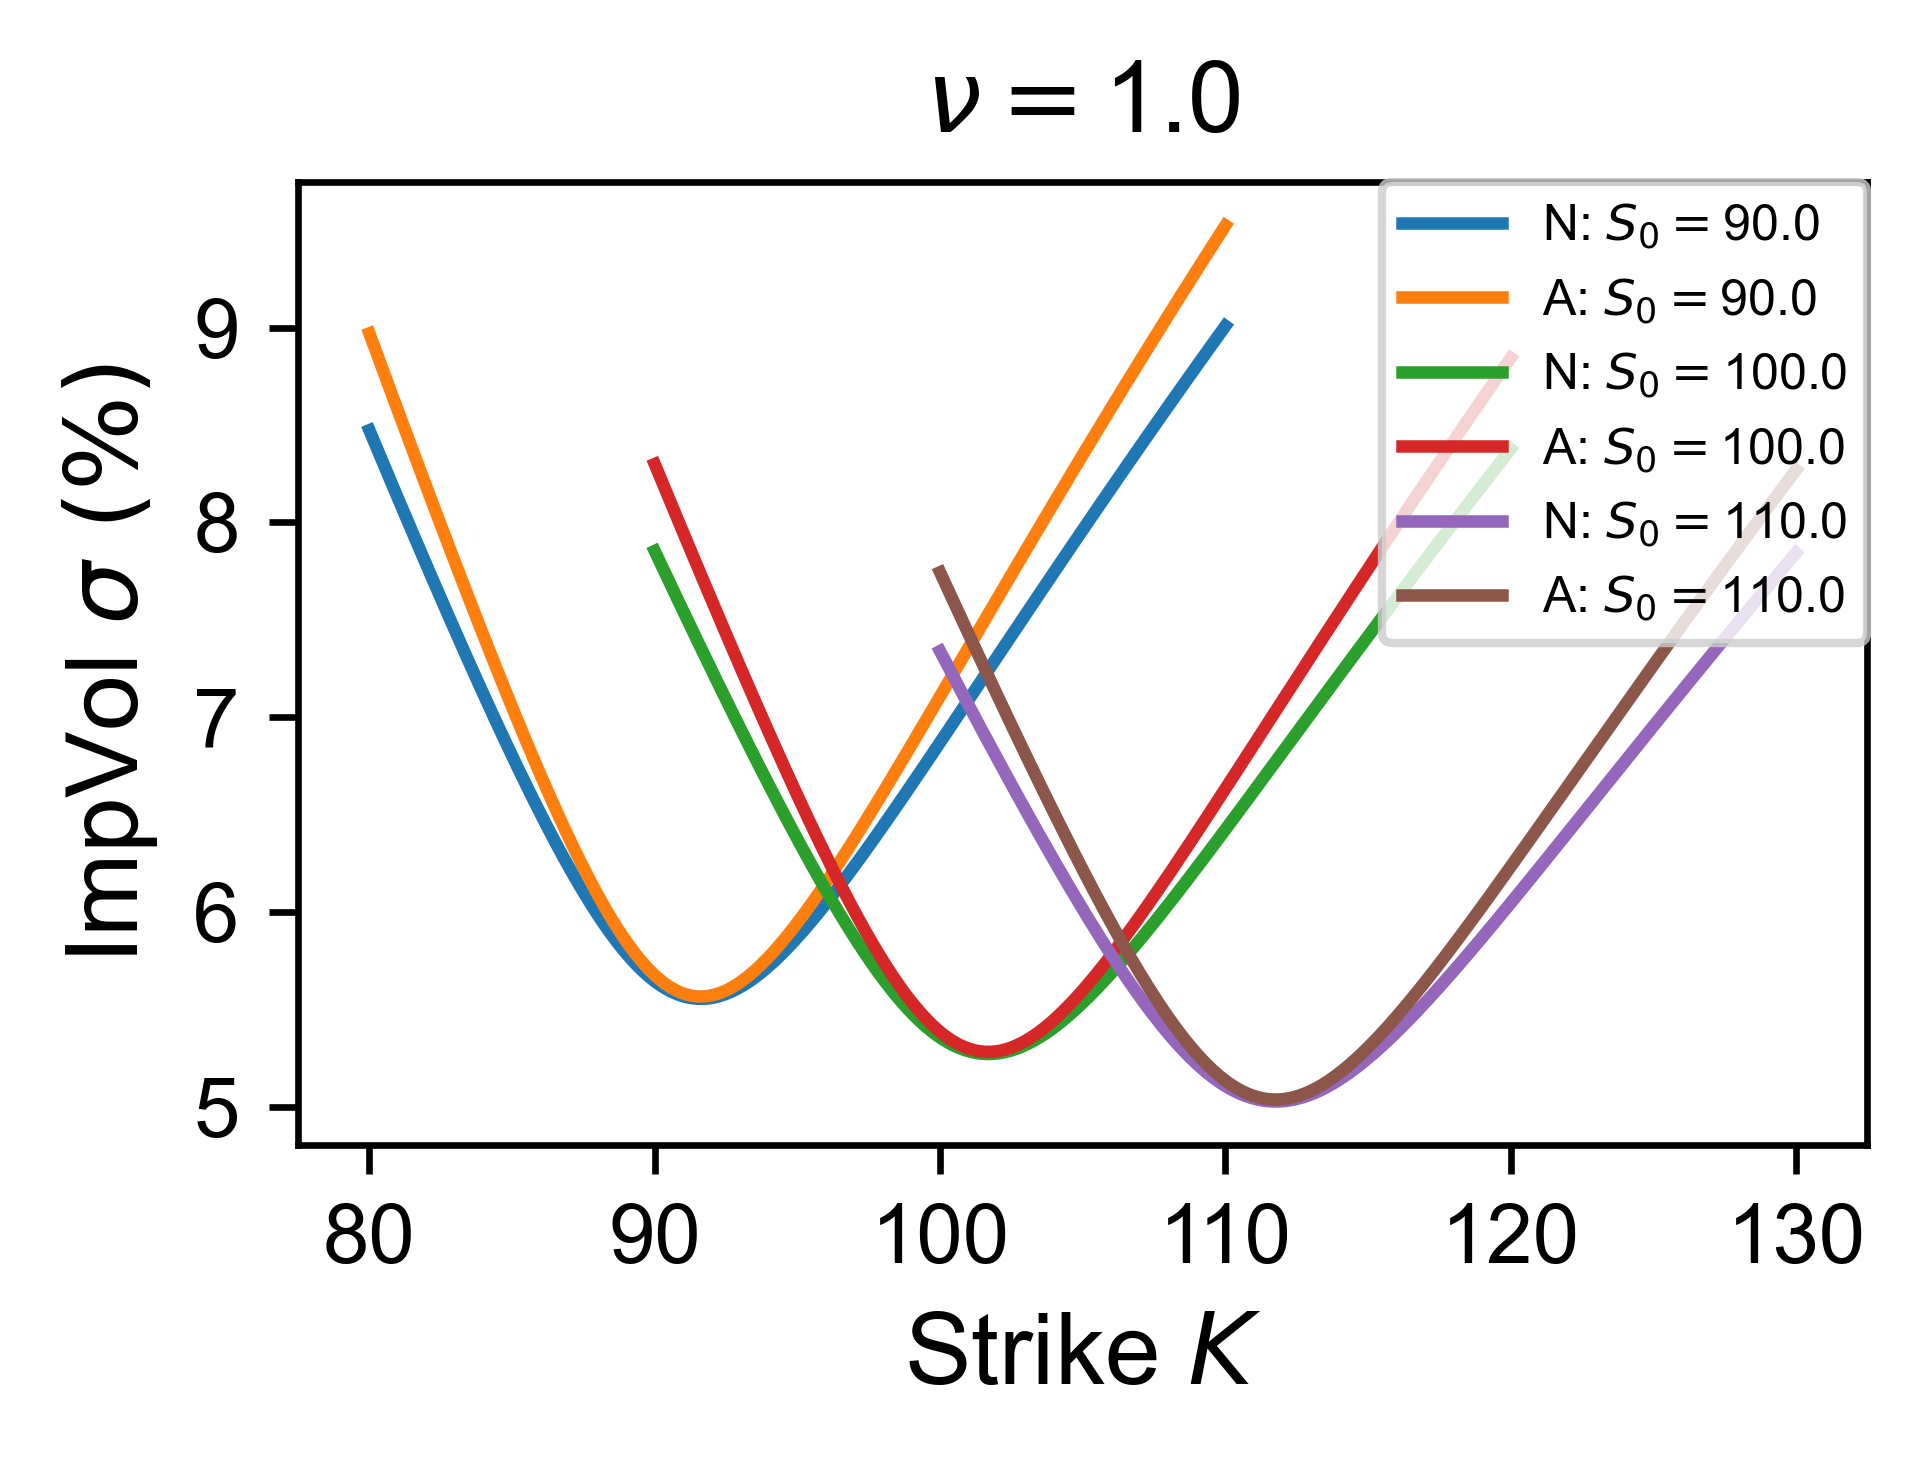
\includegraphics[width=0.7\linewidth]{image/volvol/SABR_graph_1.0.png}
    \end{minipage}
  \end{figure}

\end{frame}

\begin{frame}{SABR IVのパラメータ依存性}
  $\rho$はフォワード価格とVolの相関を表し、スキューに影響する。
  \begin{figure}
    \begin{minipage}[b]{0.48\linewidth}
      \raggedleft
      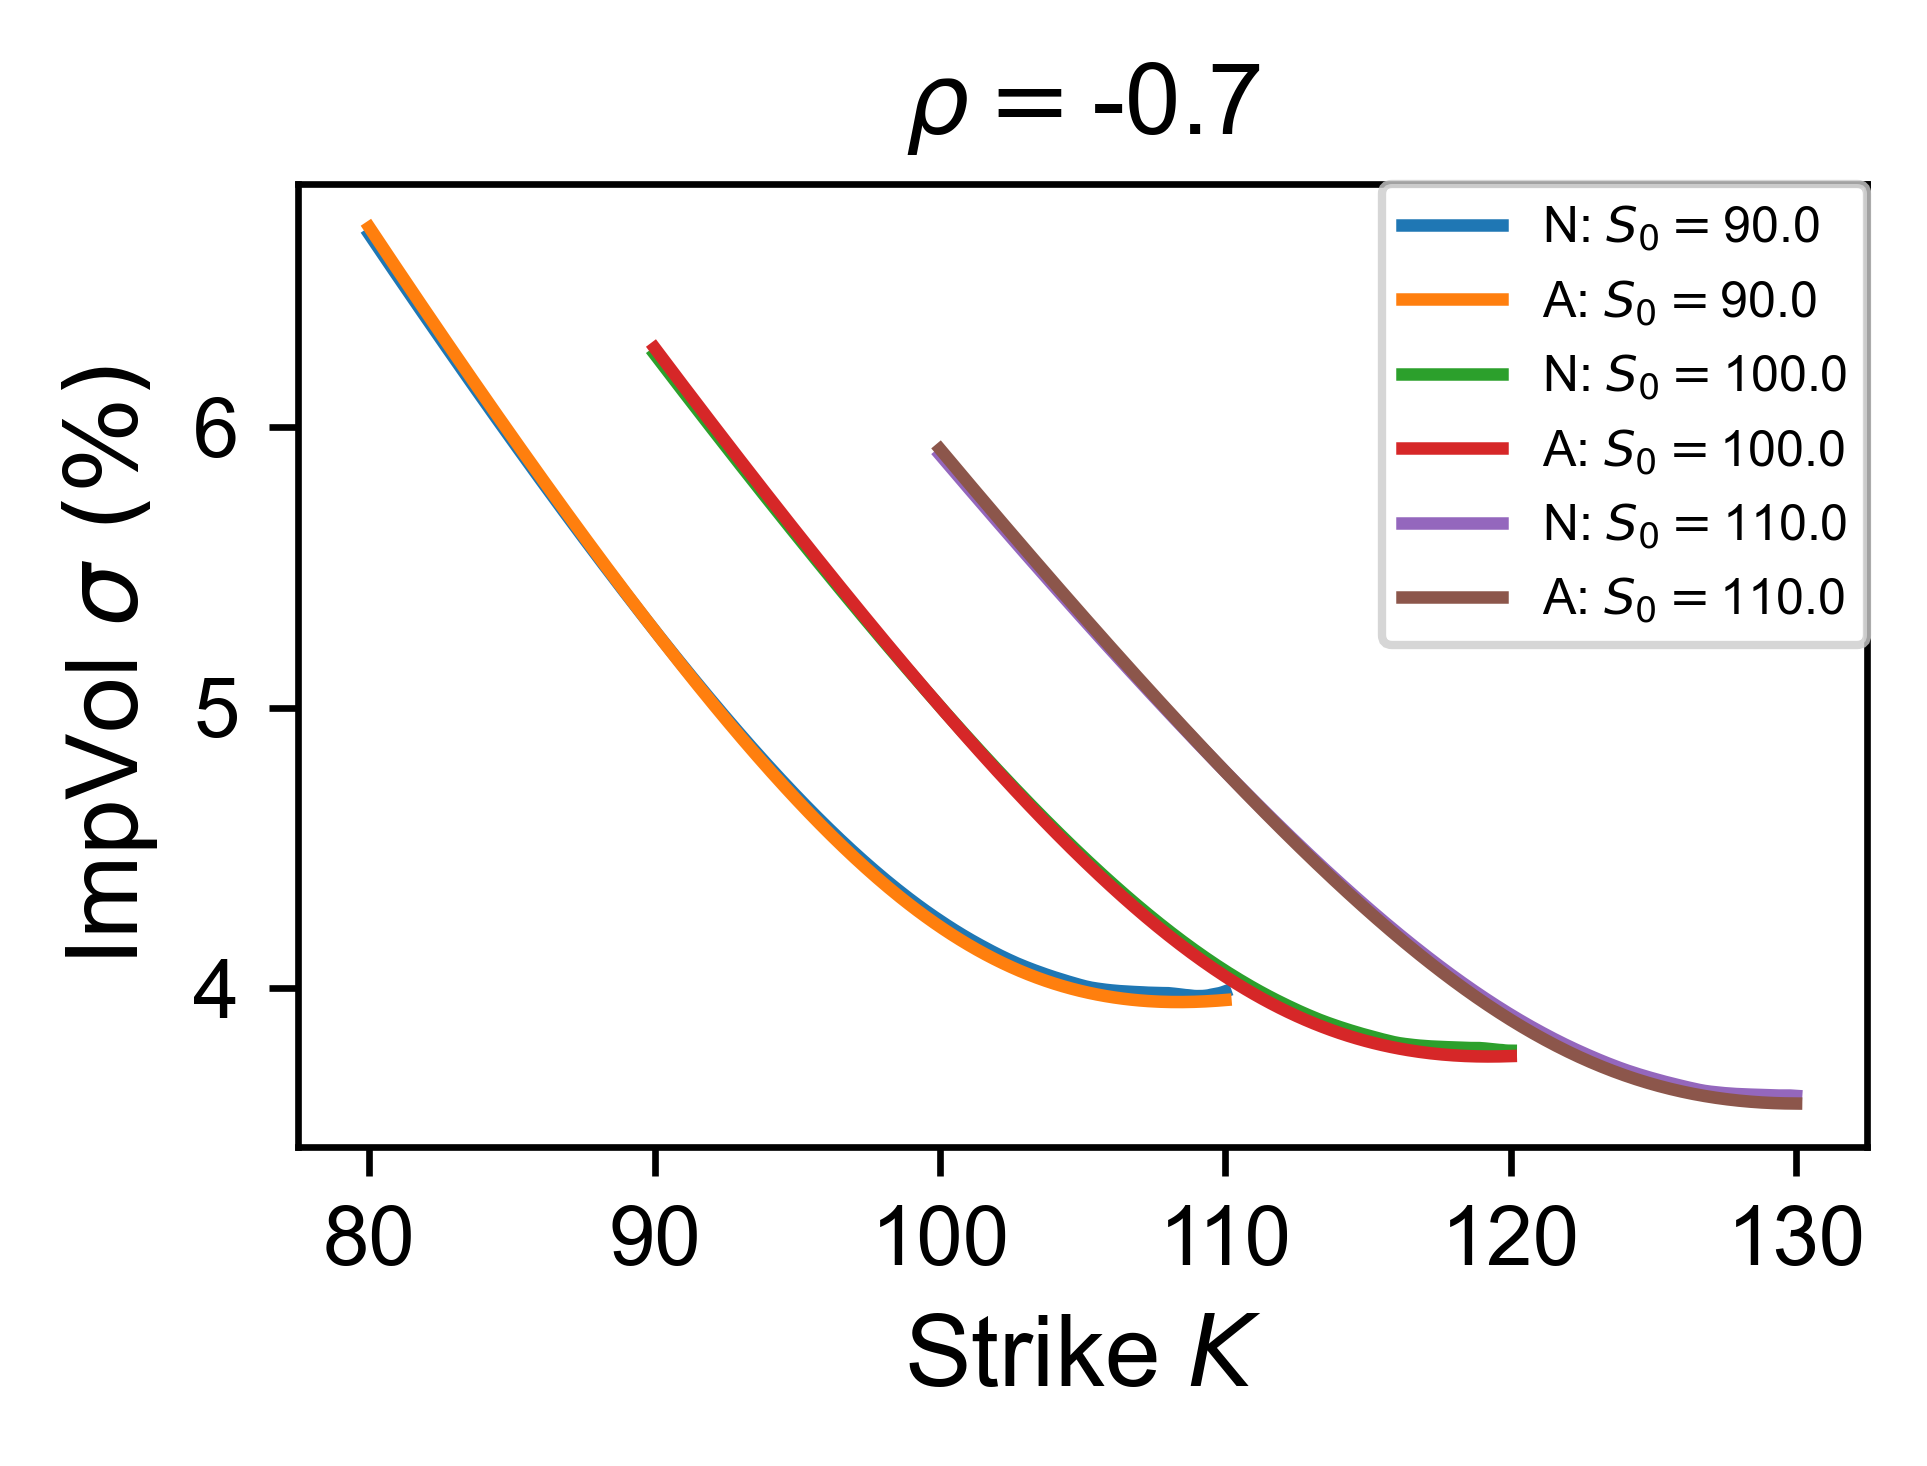
\includegraphics[width=0.7\linewidth]{image/corr/SABR_graph_-0.7.png}
    \end{minipage}
    \hfill
    \begin{minipage}[b]{0.48\linewidth}
      \raggedright
      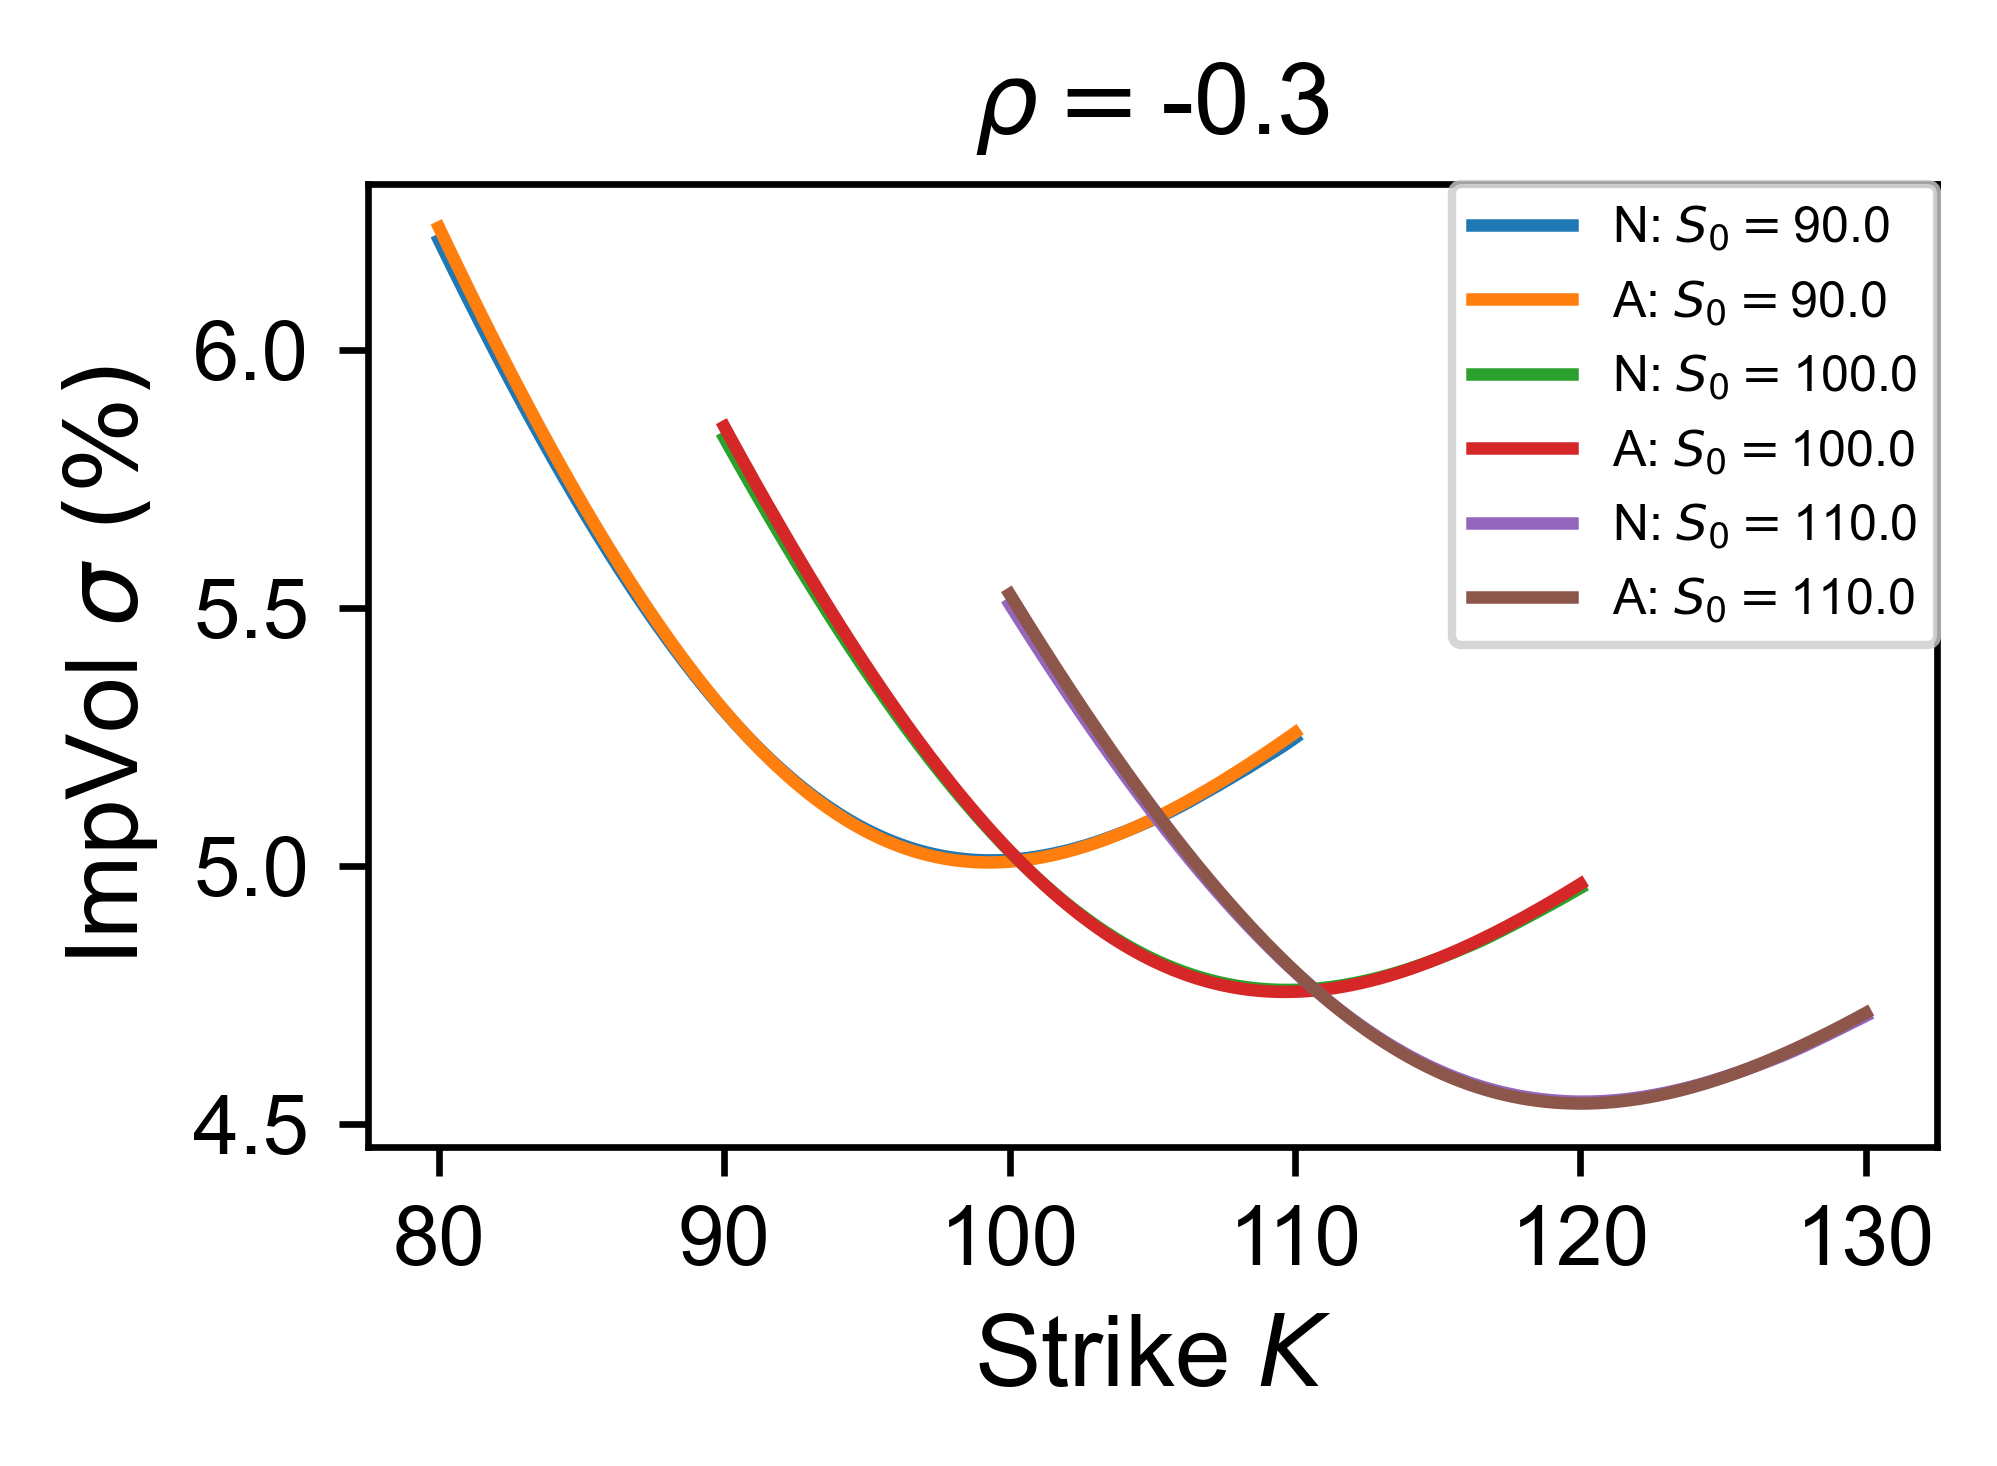
\includegraphics[width=0.7\linewidth]{image/corr/SABR_graph_-0.3.png}
    \end{minipage}
  \end{figure}

  \begin{figure}
    \begin{minipage}[b]{0.48\linewidth}
      \raggedleft
      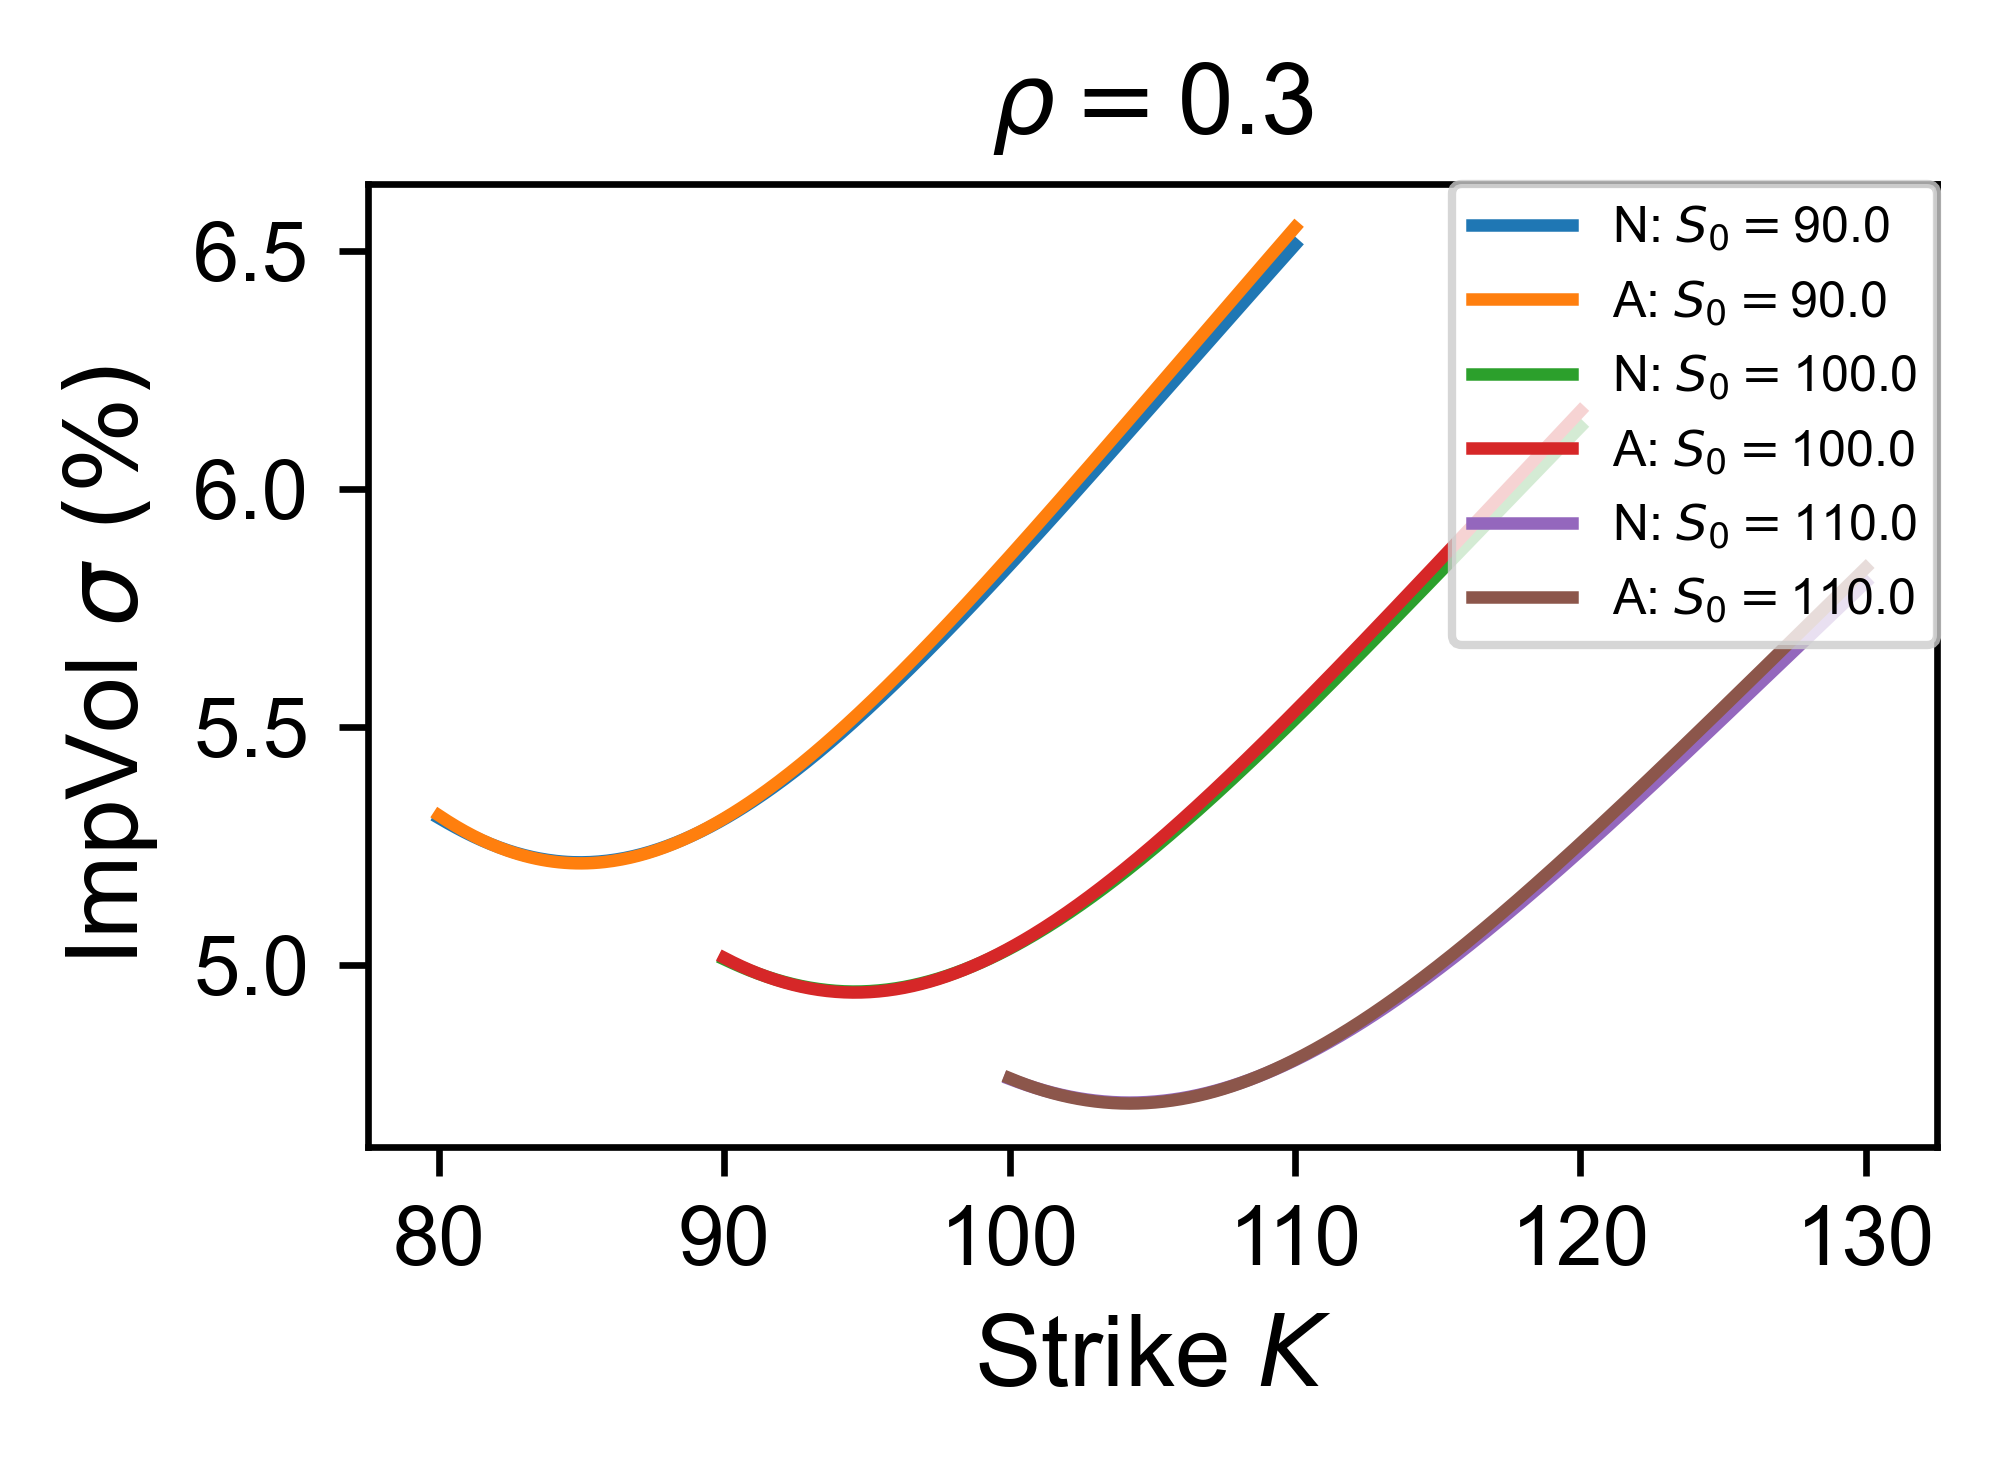
\includegraphics[width=0.7\linewidth]{image/corr/SABR_graph_0.3.png}
    \end{minipage}
    \hfill
    \begin{minipage}[b]{0.48\linewidth}
      \raggedright
      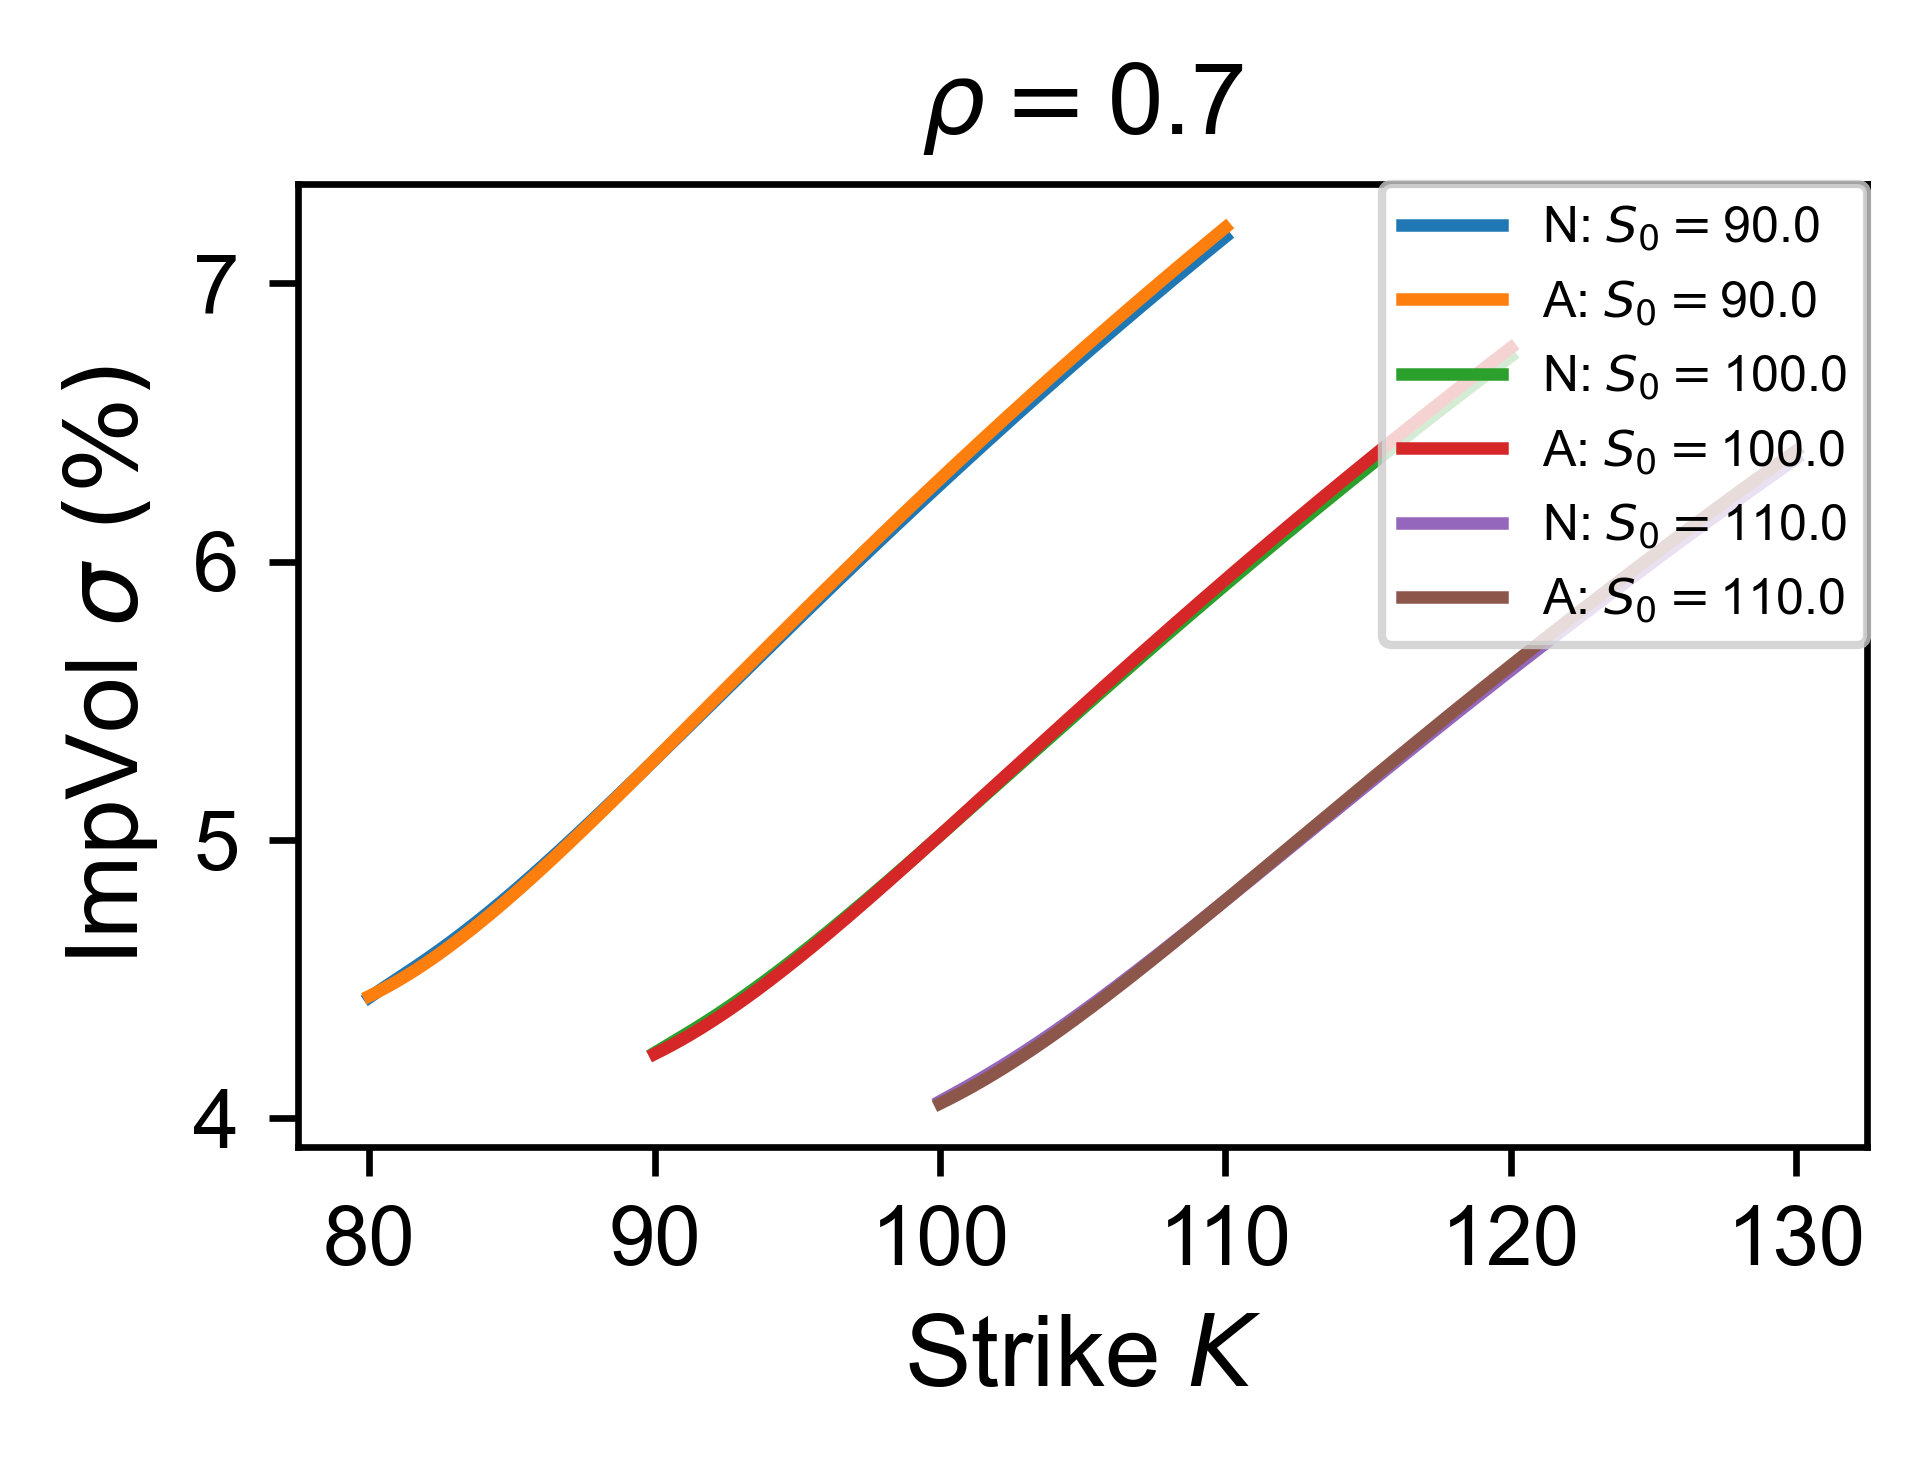
\includegraphics[width=0.7\linewidth]{image/corr/SABR_graph_0.7.png}
    \end{minipage}
  \end{figure}

\end{frame}

\subsection{Modelのrobustness}
\begin{frame}{SV Modelのrobustness}
  SV Modelを導入したのは、将来のForward価格の変動に対応するためであった。
  SABR Modelが確かに期待される振る舞いを持つことを見よう。
  $\alpha,\nu \ll 1$とすると、
  \begin{equation}
    \sigma^{IV} \simeq \frac{\alpha}{(fK)^{(1-\beta)/2}}\frac{\zeta}{x(\zeta)}
  \end{equation}
  これに対して、極小条件$\pdv{\sigma^{IV}}{K} = 0$を求めると、$\log f/K$の1次まで考えれば、
  \begin{equation}
    \zeta - \log \frac{\zeta - \rho}{1 - \rho} = 0
  \end{equation}
  これは$\zeta$だけの関数であるので、$f$の変動に伴って、$\zeta$の値を保つように極小の$K$は変わる。ここで、
  \begin{equation}
    \dd \zeta \simeq \frac{\zeta}{f} \dd f - \frac{\zeta}{K} \dd K
  \end{equation}
  であるので、フォワード価格の変動に追随して極小のストライク価格も変わることがわかる。
  \begin{alertblock}{そもそも直感的には......}
    このModelは常識的な範囲のパラメータなら、いつもATM付近でsmileの極小が見える。
    だから、$f$が変わったときに追従するのは当然といえば当然である。
  \end{alertblock}
\end{frame}

\subsection{SVにおけるGreeks}
\begin{frame}{SVにおけるGreeks}
  IVが出たので、Black Modelの解析式を用いればリスク量を算出することができる。ここでは細かいGreeksの導出は行わないが、その概略と注意点をデルタを例に見ていこう。
  \\
  直感的には、SV Modelのコールオプションの価格$C^{\mathrm{SV}}$としたとき、そのデルタは
  \begin{equation}
    \Delta = \pdv{C^{\mathrm{SV}}}{f} \overset{?}{=} \pdv{C^{\mathrm{B}}}{f} + \pdv{C^{\mathrm{B}}}{\sigma^{\mathrm{B}}} \pdv{\sigma^{\mathrm{IV}}}{f}
  \end{equation}
  とすれば良いように思われる。しかし、これは($f,\sigma^{\mathrm{B}}$以外のパラメータを定数と見ている限りにおいて)正しくない。というのも、$f$が変化すると、相関$\rho$を通じて$\alpha_{t}$(の平均)も変化するためである。この問題を解消するため、volのSDEを次のように変形する。
  \begin{equation}
    \dd \alpha_{t} = \nu \alpha_{t} \dd W_{t}^{2} = \nu\alpha_{t}\pqty{\rho \dd W_{t}^{1} + \sqrt{1-\rho^{2}} \dd Y_{t}} = g~\dd F_{t} + \nu\alpha_{t}\sqrt{1-\rho^{2}}~\dd Y_{t}
  \end{equation}
  ここで、$Y_{t}$は$W_{t}^{1}$に独立なブラウン運動であり、$g$は$F_{t}$のSDEから定まる、一般には$F_{t},\alpha_{t}$の関数となる係数である。これにより、$f$の変動による$\alpha$の変動がわかったので、正しいデルタは、
  \begin{equation}
    \Delta = \pdv{C^{\mathrm{B}}}{f} + \pdv{C^{\mathrm{B}}}{\sigma^{\mathrm{B}}} \pqty{ \pdv{\sigma^{\mathrm{IV}}}{f} + g\pdv{\sigma^{\mathrm{IV}}}{\alpha}}
  \end{equation}
  となることがわかる。
\end{frame}


\section{Exercise}
\begin{frame}{Exercise}
  SABR ModelのIVの導出方法を学んだkakuneくんは、他のModelでも同様のことができるか試したくなった。
  また同時に、SABR Modelではforward priceが大きくなったときにpriceの振動が大きくなりすぎる点を改善したくなった(本当にこれが問題たり得るのかは知らない)。
  そこで、次のようなSV Modelを考えた。
  \begin{align}
    \dd F_{t}                   & = S\frac{F_{t}^{\beta}}{F_{t}^{\beta} + \theta^{\beta}} \alpha_{t} \dd W_{t}^{1} \\
    \dd \alpha_{t}              & = \nu \alpha_{t} \dd W_{t}^{2}                                                   \\
    \dd W_{t}^{1} \dd W_{t}^{2} & = \rho \dd t
  \end{align}
  ただし、$S,\theta,\beta$は定数である($S$は不要だが、SABRの漸近展開との対応のためにつけた)。このModelに対して、IVを求めてみよう。
  \begin{enumerate}
    \item 対応する$C(f)$を書け。
    \item $z$を$f,K$を用いて書け。また、$z$を、SABRと同様に$f^{av},\log (f/K)$を用いて展開せよ。
    \item $\gamma^{(1)},\gamma^{(2)}$を求めよ。
    \item IVを求めよ。
  \end{enumerate}
  さらに、ここで求めた漸近形が正しいかどうか、数値的に確かめよう。
  \begin{enumerate}
    \setcounter{enumi}{4}
    \item $\log F_{t} , \log \alpha_{t}$についてのSDEを求めよ。
    \item 上で求めたSDEを用いて、IVを数値的に求めるプログラムを書け。
    \item 上で数値的に求めたIVと漸近形を比較し、グラフに示せ。
  \end{enumerate}

\end{frame}


\begin{frame}{Exercise:Answer}
  以下では、$\ep = 1$として解答を示す。
  \begin{enumerate}
    \item
          \begin{equation}
            C(f) =  S\frac{f}{f^{\beta} + \theta^{\beta}}
          \end{equation}
    \item
          \begin{align}
            z           & = \frac{1}{\alpha}\int_{K}^{f} \pqty{1 + \pqty{\frac{f'}{\theta}}^{-\beta}} \dd f'
            = \frac{1}{\alpha} \pqty{\pqty{f-K} + \frac{\theta^{\beta}}{1-\beta}\pqty{f^{1-\beta} - K^{1-\beta}}}                                                                                    \\
            \frac{z}{L} & \simeq f^{av}\pqty{1 + \frac{L^{2}}{24} + \frac{L^{4}}{1920}} + \theta^{\beta}(f^{av})^{1-\beta}\pqty{1 + \frac{(1-\beta)^{2}L^{2}}{24} + \frac{(1-\beta)^{4}L^{4}}{1920}}
          \end{align}
          ただし、$L = \log(f/K)$。
    \item
          \begin{equation}
            \gamma^{(1)}=\frac{\beta \theta^{\beta}}{f^{av}\pqty{(f^{av})^{\beta} + \theta^{\beta}}}, \quad
            \gamma^{(2)}=-\frac{\beta \theta^{\beta}\pqty{(1+\beta)(f^{av})^{\beta} + (1-\beta)\theta^{\beta}}}{(f^{av})^{2}\pqty{(f^{av})^{\beta} + \theta^{\beta}}^{2}}
          \end{equation}
  \end{enumerate}
\end{frame}
\begin{frame}{Exercise:Answer}
  \begin{enumerate}\setcounter{enumi}{3}
    \item
          \begin{equation}
            \phi := \pqty{2\gamma^{(2)} - (\gamma^{(1)})^{2}}(C(f^{av}))^{2}
            = -S^{2}\beta \theta^{\beta}\frac{2(1+\beta)(f^{av})^{\beta} + (2-\beta)\theta^{\beta}}{(f^{av})^{2-2\beta}\pqty{(f^{av})^{\beta} + \theta^{\beta}}^{4}}
          \end{equation}
          および$\zeta = \nu (f-K) / \alpha C(f^{av})$を使えば、解くべき方程式は、
          {\tiny
          \begin{equation}
            \frac{\sigma^{\mathrm{IV}}(f-K)}{L} \pqty{1 - \frac{(\sigma^{\mathrm{IV}})^{2}\tau^{\mathrm{ex}}}{24}} = \frac{S \alpha (f-K)}{z}\frac{\zeta}{x(\zeta)} \pqty{ 1 + \frac{\tau^{\mathrm{ex}}\alpha^{2}\phi}{24} + \frac{\tau^{\mathrm{ex}}\rho\nu\alpha\gamma^{(1)}C(f^{av})}{4} + \frac{(2-3\rho^{2})\tau^{\mathrm{ex}}\nu^{2}}{24}}
          \end{equation}
          }
          まず、最低次を求めると、$\sigma^{(0)} = S\alpha /(f^{av} + \theta^{\beta}(f^{av})^{1-\beta})$となる。これを左辺括弧内に代入して展開し、次を得る。
          \begin{equation}
            \sigma^{\mathrm{IV}} \simeq \frac{S\alpha}{z/L} \frac{\zeta}{x(\zeta)}\pqty{ 1 + \frac{\tau^{\mathrm{ex}}\pqty{\alpha^{2}\phi + (\sigma^{(0)})^{2}}}{24} + \frac{\tau^{\mathrm{ex}}\rho\nu\alpha\gamma^{(1)}C(f^{av})}{4} + \frac{(2-3\rho^{2})\tau^{\mathrm{ex}}\nu^{2}}{24}}
          \end{equation}
  \end{enumerate}
  数値計算パートのコードは、リポジトリ内にある。
\end{frame}

\end{document}
